%% FEUP THESIS STYLE for LaTeX2e
%% how to use feupteses (English version)
%%
%% FEUP, JCL & JCF, 31 July 2012
%%
%% PLEASE send improvements to jlopes at fe.up.pt and to jcf at fe.up.pt
%%

%%========================================
%% Commands: pdflatex tese
%%           bibtex tese
%%           makeindex tese (only if creating an index) 
%%           pdflatex tese
%% Alternative:
%%          latexmk -pdf tese.tex
%%========================================

\documentclass[11pt,a4paper,twoside,openright]{report}

%% My packages
\usepackage{amssymb}
\usepackage{multirow}
\usepackage{multicol}
\usepackage{caption}
\usepackage{fancyvrb}
\usepackage{subcaption}
\usepackage{url}
\usepackage[intoc]{nomencl}
\usepackage{array}

%% For iso-8859-1 (latin1), comment next line and uncomment the second line
\usepackage[utf8]{inputenc}
%\usepackage[latin1]{inputenc}

%% English version

%% MIEIC options
%\usepackage[mieic]{feupteses}
\usepackage[mieic,juri,backrefs]{feupteses}
%\usepackage[mieic,final]{feupteses}
%\usepackage[mieic,final,onpaper]{feupteses}

%% Additional options for feupteses.sty: 
%% - onpaper: links are not shown (for paper versions)
%% - backrefs: include back references from bibliography to citation place

%% Uncomment the next lines if side by side graphics used
%\usepackage[lofdepth,lotdepth]{subfig}
%\usepackage{graphicx}
%\usepackage{float}

%% Include color package
\usepackage{color}
\definecolor{cloudwhite}{cmyk}{0,0,0,0.025}

%% Include source-code listings package
\usepackage{listings}
\lstset{ %
 language=C,                        % choose the language of the code
 basicstyle=\footnotesize\ttfamily,
 keywordstyle=\bfseries,
 numbers=left,                      % where to put the line-numbers
 numberstyle=\scriptsize\texttt,    % the size of the fonts that are used for the line-numbers
 stepnumber=1,                      % the step between two line-numbers. If it's 1 each line will be numbered
 numbersep=8pt,                     % how far the line-numbers are from the code
 frame=tb,
 float=htb,
 aboveskip=8mm,
 belowskip=4mm,
 backgroundcolor=\color{cloudwhite},
 showspaces=false,                  % show spaces adding particular underscores
 showstringspaces=false,            % underline spaces within strings
 showtabs=false,                    % show tabs within strings adding particular underscores
 tabsize=2,	                    % sets default tabsize to 2 spaces
 captionpos=b,                      % sets the caption-position to bottom
 breaklines=true,                   % sets automatic line breaking
 breakatwhitespace=false,           % sets if automatic breaks should only happen at whitespace
 escapeinside={\%*}{*)},            % if you want to add a comment within your code
 morekeywords={*,var,template,new}  % if you want to add more keywords to the set
}

%% Uncomment to create an index (at the end of the document)
%\makeindex

%% Path to the figures directory
%% TIP: use folder ``figures'' to keep all your figures
\graphicspath{{figures/}}

\makenomenclature
\renewcommand{\nomentryend}{.}
\renewcommand{\nomlabel}[1]{\hfil\textbf{#1}}

%%----------------------------------------
%% TIP: if you want to define more macros, use an external file to keep them
%some macro definitions

% format
\newcommand{\class}[1]{{\normalfont\slshape #1\/}}

% entities
\newcommand{\Feup}{Faculdade de Engenharia da Universidade do Porto}

\newcommand{\svg}{\class{SVG}}
\newcommand{\scada}{\class{SCADA}}
\newcommand{\scadadms}{\class{SCADA/DMS}}

%%----------------------------------------

%%
%% Hyperlinks
%%

% MiniTOC
\usepackage[tight]{minitoc}

\dominitoc
\renewcommand{\mtctitle}{}
\renewcommand{\kernafterminitoc}{\vspace{0.3cm}}
\renewcommand{\mtcoffset}{-0.3cm}
%\setcounter{minitocdepth}{1}

%%========================================
%% Start of document
%%========================================
\begin{document}

%%----------------------------------------
%% Information about the work
%%----------------------------------------
\title{Social Media Text Processing and Semantic Analysis for Smart Cities}
\author{João Filipe Figueiredo Pereira}

%% Uncomment next line for date of submission
%\thesisdate{July 31, 2008}

%%Uncomment next line for copyright text if used
%\copyrightnotice{Name of the Author, 2008}

\supervisor{Supervisor}{Rosaldo José Fernandes Rossetti}
\supervisor{Co-supervisor}{Pedro dos Santos Saleiro da Cruz}


%% Uncomment next line if necessary
%\supervisor{Second Supervisor}{Name of the Supervisor}

%% Uncomment committee stuff in the final version if used
%\committeetext{Approved in oral examination by the committee:}
%\committeemember{Chair}{Doctor Name of the President}
%\committeemember{External Examiner}{Doctor Name of the Examiner}
%\committeemember{Supervisor}{Doctor Name of the Supervisor}
%\signature

%% Specify cover logo (in folder ``figures'')
\logo{uporto-feup.pdf}

%% Uncomment next line for additional text  below the author's name (front page)
%\additionalfronttext{Preparação da Dissertação}

%%----------------------------------------
%% Preliminary materials
%%----------------------------------------

% remove unnecssary \include{} commands
\begin{Prolog}
  \chapter*{Abstract}

With the rise of Social Media, people obtain and share information almost instantly on a 24/7 basis. Many research areas have tried to gain valuable insights into these large volumes of freely available user generated content. The research areas of intelligent transportation systems and smart cities are no exception. However, extracting meaningful and actionable knowledge from user generated content is a complex endeavor. First, each social media service has its own data collection specificities and constraints, second the volume of messages/posts produced can be overwhelming for automatic processing and mining, and last but not the least, social media texts are usually short, informal, with a lot of abbreviations, jargon, slang and idioms.
 
In this thesis, we try to tackle some of the aforementioned challenges with the goal of extracting knowledge from social media streams that might be useful in the context of intelligent transportation systems and smart cities. We designed and developed a framework for collection, processing and mining of geo-located Tweets. More specifically, it provides functionalities for parallel collection of geo-located tweets from multiple pre-defined bounding boxes (cities or regions), including filtering of non complying tweets, text pre-processing for Portuguese and English language, topic modeling, and transportation-specific text classifiers, as well as, aggregation and data visualization.

To build our transportation-specific text classifiers, we take support of the recent advances of text mining techniques, such as word embeddings. Our experiments prove that using word embedding features to fed into our models training phase, robustness and generalization are achieved in the classification task. For instance, tweets about transport-modes (e.g. "Uber") that are not considered in the models training process, are discriminated as travel-related tweets by our classification models.

We performed empirical studies and implemented illustrative examples for 5 cities: Rio de Janeiro, São Paulo, New York City, London and Melbourne, comprising a total of more than 43 millions tweets in a period of 3 months. The topic modeling and text classifiers were evaluated with manual labeled data specifically created for this work. Both software and gold standard data will be made publicly available to foster further developments from the research community.


\chapter*{Resumo}

Devido à ascensão das Redes Sociais, as pessoas obtêm e partilham informação quase que instantaneamente 24/7. Muitas áreas de investigação tentaram extrair informações importantes destes grandes volumes de conteúdo, gerado por utilizadores, e livremente disponíveis. As áreas de investigação de sistemas inteligentes de transportes e de cidades inteligentes (\textit{smart cities}) não são excepção. Contudo, extrair conhecimento acionável e significativo de conteúdo gerado por utilizadores exige um esforço complexo. Primeiro, cada serviço de social media possui as suas próprias especificidades e restrições para o método de recolha dos dados; em segundo lugar, o volume de mensagens produzidas pode ser esmagador para o processamento automático e prospeção; e por último, não menos importante, os textos das redes sociais são, geralmente, curtos, informais, com muitas abreviações, jargões, gírias e expressões idiomáticas. 

Nesta dissertação, tentamos abordar alguns dos desafios acima mencionados com o objectivo de extrair conhecimento de mensagens das redes sociais que possam ser úteis no contexto de sistemas inteligentes de transportes e cidades inteligentes (\textit{smart cities}). Nós idealizamos e desenvolvemos uma \textit{framework} para a recolha de dados, processamento e prospeção de Tweets geo-localizados. Mais especificamente, a \textit{framework} fornece funcionalidades para a recolha paralela de tweets geo-localizados de \textit{bounding-boxes} (cidades ou regiões), incluindo filtragem de tweets não preenchidos, pré-processamento de texto para a língua portuguesa e inglesa, modelagem de tópicos e classificadores de texto específicos para transportes, bem como, agregação e visualização de dados.

Realizamos estudos empíricos e implementamos exemplos ilustrativos para 5 cidades: Rio de Janeiro, São Paulo, Nova York, Londres e Melbourne, perfazendo um total de mais de 43 milhões de tweets em um período de 3 meses. O modelo de tópicos e os classificadores de texto foram avaliados com dados manualmente anotados e criados especificamente para este trabalho. Tanto os dados quanto o software criados serão disponibilizados publicamente para promover novos desenvolvimentos da comunidade de investigação. % the abstract
  \chapter*{Acknowledgements}

Aliquam id dui. Nulla facilisi. Nullam ligula nunc, viverra a, iaculis
at, faucibus quis, sapien. Cum sociis natoque penatibus et magnis dis
parturient montes, nascetur ridiculus mus. Curabitur magna ligula,
ornare luctus, aliquam non, aliquet at, tortor. Donec iaculis nulla
sed eros. Sed felis. Nam lobortis libero. Pellentesque
odio. Suspendisse potenti. Morbi imperdiet rhoncus magna. Morbi
vestibulum interdum turpis. Pellentesque varius. Morbi nulla urna,
euismod in, molestie ac, placerat in, orci. 

Ut convallis. Suspendisse luctus pharetra sem. Sed sit amet mi in diam
luctus suscipit. Nulla facilisi. Integer commodo, turpis et semper
auctor, nisl ligula vestibulum erat, sed tempor lacus nibh at
turpis. Quisque vestibulum pulvinar justo. Class aptent taciti
sociosqu ad litora torquent per conubia nostra, per inceptos
himenaeos. Nam sed tellus vel tortor hendrerit pulvinar. Phasellus
eleifend, augue at mattis tincidunt, lorem lorem sodales arcu, id
volutpat risus est id neque. Phasellus egestas ante. Nam porttitor
justo sit amet urna. Suspendisse ligula nunc, mollis ac, elementum
non, venenatis ut, mauris. Mauris augue risus, tempus scelerisque,
rutrum quis, hendrerit at, nunc. Nulla posuere porta orci. Nulla dui. 

Fusce gravida placerat sem. Aenean ipsum diam, pharetra vitae, ornare
et, semper sit amet, nibh. Nam id tellus. Etiam ultrices. Praesent
gravida. Aliquam nec sapien. Morbi sagittis vulputate dolor. Donec
sapien lorem, laoreet egestas, pellentesque euismod, porta at,
sapien. Integer vitae lacus id dui convallis blandit. Mauris non
sem. Integer in velit eget lorem scelerisque vehicula. Etiam tincidunt
turpis ac nunc. Pellentesque a justo. Mauris faucibus quam id
eros. Cras pharetra. Fusce rutrum vulputate lorem. Cras pretium magna
in nisl. Integer ornare dui non pede. 

\vspace{10mm}
\flushleft{The Name of the Author}
  % the acknowledgments
  \cleardoublepage
\thispagestyle{plain}

\vspace*{8cm}

\begin{flushright}
   \textsl{``You should be glad that bridge fell down. \\
           I was planning to build thirteen more to that same design''} \\
\vspace*{1.5cm}
           Isambard Kingdom Brunel
\end{flushright}
       % initial quotation if desired
  \cleardoublepage
  \pdfbookmark[0]{Table of Contents}{contents}
  \tableofcontents
  \cleardoublepage
  \pdfbookmark[0]{List of Figures}{figures}
  \listoffigures
  \cleardoublepage
  \pdfbookmark[0]{List of Tables}{tables}
  \listoftables
  \chapter*{Abbreviations}
\chaptermark{ABBREVIATIONS}

\begin{flushleft}
\begin{tabular}{l p{0.8\linewidth}}
SC      & Smart City \\
SM		& Smart Mobility \\
ITS      & Intelligent Transportation System \\
ICT		& Information and Communication Technology \\
SMA		& Social Media Analytics \\
HTTP	& Hypertext Transfer Protocol \\
TSL		& Transport Security Layer \\
POS		& Part-of-speech \\
BoW		& Bag-of-words \\
VSM		& Vector Space Model \\
LDA		& Latent Dirichlet Allocation \\
CRF		& Conditional Random Fields \\
HHM		& Hidden Markov Model \\
ABSA	& Aspect-based Sentiment Analysis \\
SSWE	& Sentiment Specific Word Embeddings \\
ML		& Machine Learning \\
SVM		& Support Vector Machines \\
NB 		& Naïve Bayes \\
ME		& Maximum Entropy \\
RF		& Random Forests \\
DL		& Deep Learning \\
MAE		& Mean Absolute Error \\
OLS		& Ordinary Least Squares \\
LR		& Logistic Regression
\end{tabular}
\end{flushleft}

  % the list of abbreviations used
\end{Prolog}

%%----------------------------------------
%% Body
%%----------------------------------------
\StartBody

%% TIP: use a separate file for each chapter
\chapter{Introduction} \label{chap:intro}

\minitoc \mtcskip \noindent

\section{Context and Motivation}\label{sec:context_motivation}

In the last few years, the rise of Web 2.0, seen as the evolution of conventional Web services into collaborative and social platforms~\cite{chi2008social}, conducted to an excessive amount of User Generated Content~\cite{kaplan2010users} (UGC) being placed \textit{online} by the population. Due to this emergency of web-content, the research community has been exploring it in order to extract added-value information regarding a large diversity of domains, such as opinion mining, human behavior and respective activity patterns, political issues, social communication (e.g. news websites). Social media platforms, more specifically, social media content (SMC), a type of UGC, has been targeted by several scientific researches focused mostly in the text mining area. Although the application of SMC in the previous mentioned domains, the \textit{smart cities}~\cite{batty2012smart} and, in particular, the transportation~\cite{gal2014potential} domain are under a smooth growth, meaning that a large path is still unexplored allowing new opportunities and challenges for the research community to reach its full potential~\cite{kn:Musto2015}.

Availability and authenticity are some of the social media content advantages considering that such information do not require additional costs regarding its exploration, is, \textit{a priori}, generated by humans, transcending a certain level of credibility and, lastly, due to the availability of tools provided by social media platforms, we can store the data and perform off-line analysis~\cite{kuflik2017automating}. Twitter is considered a MicroBlog, a type of social network, which content is similar to SMS-like messages, characteristic of a 140-characters length, and the 11th most visited website in the world~\footnote{http://www.alexa.com/siteinfo/twitter.com}. This platform has already proved its value and potential in domains ranging from news detection~\cite{kn:Sankaranarayanan2009} to real-time traffic sensing~\cite{carvalho2010real} being for this reason one of the most explored sources of data during the conduction of research studies.

Mining Twitter data is although the availability and free cost, a laborious and time-consuming process due to the restrictions and difficulties present in its content. The informal language, the existence of slang, abbreviations, jargons and the short length of the message are some of the problems when analyzing this data. Harvesting tweets automatically and, at the same time, extracting valuable information for the target domains delineated in this dissertation makes the task even more complex. However, by surpassing the previous mentioned problems, the extracted information may be of extremely importance and useful to the final stakeholders, namely \textit{smart cities} and transportation entities, during decision-making policies to improve their services.

\section{Problem Statement}\label{sec:problem}
The problem around this dissertation is focused in the analysis of a continuous flow of social media streams provided by Twitter. To analyse such streams, multiple steps composed in an iterative process are needed in order to filter out non-related content and proceed with extraction of information about a specific scenario. Here, since the target scenarios are associated to \textit{smart cities} and transportation domains, data related to it must be explored and analysed. To the best of our knowledge, there are no public datasets related to these domains and the creation of a gold standard dataset constitutes a complex endeavor, which is, for this reason, an obstacle to surpass in this dissertation. The extraction of information from social media content is another overwhelming task since it is necessary the application of several NLP methods in order to minimize/extinct its peculiarly problems. Hence, the main problem can be divided in five distinct sub-problems:

\begin{enumerate}
	\item \textbf{Data collection method for various locations}\\
	Choosing a method to collect data that provides a large range of valuable information for different cities constitutes the first sub-problem.
	
	\item \textbf{Content filtering}\\
	It is necessary the guarantee of that all information is fully related to the target scenario in the analysis, as well as removing messages which does not brought additional information (for instance, tweets only composed by \textit{emoticons}) or are not related to the end-users expectations, i.e. if we are targeting content from a specific city, we must assure that such content is indeed posted when users were there.
	
	\item \textbf{Identification of topics in Twitter messages}\\
	The identification of topics in Twitter messages is a very important point in the analyses of the \textit{smart cities} context. This task allows the identification of what is been talked about recently and also where the conversation topics are geographically distributed.
	
	\item \textbf{Travel-related classification}\\
	In order to produce valuable information for the transportation services, we need to analyse the content of a message and verify if it is truly related with the domain in study. Hence, discriminate travel-related tweets is one of the sub-problems that must be tackled.
	
	\item \textbf{Data aggregation and visualization}\\
	The aggregation of the results provide by all other tasks is needed. This aggregation task may be continuously calculating the results in order to make the user experience easier and smooth without taking to much response time by the data visualization UI. The graphical visualizations should be of easy interpretation by the end-user and having this in mind some qualitative and quantitative indicators may be presented.
\end{enumerate}

\section{Goals and Expected Contributions}\label{sec:contributions}
Following the previous mentioned problem in Section \ref{sec:problem}, the main goal of this dissertation passes through the development of a prototype framework based on the concept of analysis. Such framework demands a solution for each of the aforementioned sub-problems, and for that reason modularity is needed in the design and implementation of the final tool. Its usability will be directed to companies or even ordinary users and should be able to provide relevant information about a specific real-world scenario under the \textit{smart cities} and transportation fields. The framework should be capable of automatically processing social media texts, more specifically, general topic detection and characterization of travel-related tweets. The following list summarizes the crucial goals behind this dissertation:

\begin{itemize}
	\item Extraction of valuable information from Social Media Content to the Transportation and \textit{Smart Cities} domains;
	\item Designing and implementation of a framework capable of automatize the analysis process;
	\item Application, when possible, of recent advances in the area of text analysis;
\end{itemize}

\medskip

In terms of expected contributions, we hope that such generated information through the framework data analytics may be relevant both to ordinary users of a particular service and to the responsible entities in order to improve decision-making policies.

\section{Publications}\label{sec:publications}
In this section several scientific contributions performed during the period of this dissertation are mentioned:

\begin{itemize}
		\item
		João Pereira, Arian Pasquali, Pedro Saleiro and Rosaldo J. F. Rossetti. {\color{blue}Transportation in Social Media: an automatic classifier for travel-related tweets}. In \emph{Portuguese Conference on Artificial Intelligence} (EPIA), 2017. In Press.
		
		\item
		João Pereira, Arian Pasquali, Pedro Saleiro and Rosaldo J. F. Rossetti. {\color{blue}Classifying Travel-related Tweets using Word Embeddings}. In \emph{International Conference on Information and Knowledge Management} (CIKM), 2017. Under review.
		
		\item
		João Pereira, Arian Pasquali, Pedro Saleiro and Rosaldo J. F. Rossetti. {\color{blue}Characterizing Geo-located Tweets in Brazilian Megacities}. In \emph{IEEE International Summer School on Smart Cities} (IEEE S3C), 2017. Under review.
\end{itemize}

\section{Dissertation Structure}\label{sec:diss_structure}
The effort applied to this dissertation generated a great diversity of points and due to that the remainder of the document is structured into four chapters.
Section \ref{chap:sota} starts with a brief conceptualization in the Smart Cities and Intelligent Transportation System domains, as well as previous related works using social media content as its basis.
The proposed framework is referenced in Section \ref{chap:framework}, being each its composing modules depth described.
Experiments performed to test each module of the framework are reported in Section~\ref{chap:experiments}.
Completing this document, conclusions, future work and a few final remarks are exposed in chapter~\ref{chap:conclusions}.
\chapter{Introduction} \label{chap:intro}

\minitoc \mtcskip \noindent

\section{Context and Motivation} \label{sec:context}
The rise of social media services, in the last few years, has led to an excessive amount of information being placed online by the population. The need to explore this type of information has a steadily grown in order to realize what kind of value could bring to the areas of marketing, business or even politician \cite{kn:Feldman:2013}. Micro-blogging platforms, such as Twitter, have a huge affluence in a daily-basis, where people publicly share around 500 million messages about a diverse set of current themes, expressing their opinions and feelings \cite{kn:Giachanou2016}. For this reason, technological projects developed in some cities has seen social media streams as a potential resource to extract knowledge, i.e. the satisfaction of people regarding some services in the cities, such as the urban transportation service \cite{kn:Anastasi2013}. The collection of this participative activity of people through online platforms, named Crowd Sensing, emerged to replace the traditional way of sensing data capture and tracking in physical infrastructures, allowing a considerable reduction of economic costs \cite{kn:Szabo2013}.

The information extraction from social media streams is a hard task. For example, tweets besides being text messages and, consequently unstructured data. There's also some extra particularities, as, for example, the limited length (140 characters per message) which restricts the amount of information in its content, the informal language used and there are also many spell-mistakes, abbreviations, ambiguity and special mentions (e.g. URL references, hashtags, users) and the presence of a high variety of emoticons \cite{kn:Musto2015}.

Many research projects have been conducted in order to extract the sentiment present in opinions through text mining techniques. Sentiment analysis is the field that focuses on this task. The detection of the sentiment polarity in messages generated by citizens, whether at a specific level (relative to certain aspects) or at a general level (general sentiment of the message) can allow companies or even ordinary citizens the possibility of identification city's services problems and may be assimilated to a kind of sensor for the issue of quality awareness, providing, at least, some help in decision-making processes.

\section{Problem Statement and Goals} \label{sec:problemstatement_goals}
The problem around this dissertation establishes in the analysis of a continuous flow of social media streams, in particular from Twitter, about a target scenario, as, for example, the quality of the urban transportation services in Porto. Hence, it will be necessary to filter the relevant messages, extract sentiment aspects/topics with polarity and create useful aggregated data visualizations. The problem presented can be divided in five distinct points:

\begin{enumerate}
\item \textbf{Data collection for our target scenario}

At this point, a real scenario must be chosen so that a case study can be produced.

\item \textbf{Named Entity Disambiguation and content filtering}

The identification of the entities present in the messages is a important point in order to disambiguate some mentions that could not be related with target scenario, making the filtering task easier, since only messages that are related must appear in the final dataset.

\item \textbf{Identification of aspects/topics in Twitter messages}

Since each opinion usually has a target aspect/topic about an entity, or even a service of a city, the recognition of it is relevant so that the sentiment present in the message has an orientation.

\item \textbf{Sentiment polarity classification}

The polarity of a sentiment may have three different types: positive, negative or neutral. At this point, it will be necessary to estimate the level of polarity expressed in the message.

\item \textbf{Data aggregation and visualization}

The aggregation of the results provide by all other tasks is needed. Some messages could refer to the same aspect through different ways, so it will be  necessary aggregate messages that present this characteristic. Another important task of the aggregation is the continuously calculation of the results So that when an user access the analytics UI, the results are presented immediately, without waiting time. At the visualization of the results, some qualitative and quantitative indicators may be presented to the end-user to make the analysis easier.

\end{enumerate}

Taking into account all the aforementioned points, the final goal of this dissertation is to create a framework, based on the concept of analysis. The framework should be capable of automatically processing social media texts, regarding semantic processing, topic detection and sentiment analysis. An user interface will be provide to the end-user, illustrating a set of qualitative and quantitative indicators to analysis. This knowledge can be relevant both to users of a particular service or to the responsible entities in order to improve the decision-making process.

\section{Structure of this Dissertation} \label{sec:struct}
This report covers a great diversity of points and because of that, its structure is divided in three different sections.

The Section \ref{chap:sota} starts with a brief contextualization in the Smart Cities and Intelligent Transportation System fields. After that, it was made a review on Social Media Analytics, specially about Twitter, and what benefits its exploration can provide to the civilization. To explore the information from Twitter messages, an intensive study regarding the Text Mining area was made, in particular Information Extraction, Topic Modeling and the various Sentiment Analysis fields, as well as related works that already explored similar problems with social media data.

The proposed solution for the aforementioned problem and its methodology are referenced in Section \ref{chap:problemsolution}. The final section of this planning report is composed by some conclusions relatively to the studied works and what benefits and risks our solution may have - Section \ref{chap:conclusions}.

%Para além da introdução, esta dissertação contém mais x capítulos.
%No capítulo~\ref{chap:sota}, é descrito o estado da arte e são
%apresentados trabalhos relacionados.

\chapter{Old Background and Literature Review} \label{chap:sota}

\minitoc \mtcskip \noindent

This section aims the analysis and reflection about some works and topics that will be relevant to fully understand the problem. The study of solutions found by other authors can simplify the difficult task that is the analysis of social media data.
Hence, this section has been divided into several parts in order to perceive not only the environment in which the problem is located but also the most important points to be studied in order to build our the final product. Respectively to the problem scope its important to know what is a smart city and how the transportation system can contribute to this meaning. Since our product is a framework which goal is to extract information about social media data, i.e. texts from the Twitter, its interesting obtain the knowledge about extraction tools, such as the Twitter APIs, in order to have an idea how to construct our crawler module. The meaning of text mining and how the information present in texts can be extracted through different kinds of techniques, regarding disambiguation, filtering and modeling. Finally, it is also important to analyze several works about sentiment analysis in order to know the different methodologies and which are the most advantageous for this problem.

\section{Smart Cities and Intelligent Transportation Systems}\label{sec:smartcities}

The Smart City concept appeared thanks to the continuous growth of a city's population which has contributed to an aggressive urbanization \cite{kn:Cecilia2016}. In the last few years, several definitions for its meaning have emerged, but the ideal one is not yet fully known. Angelidou in \cite{kn:Angelidou2015} defines Smart City as a "conceptual urban development model on the basis of the utilization of human, collective, and technological capital for the development of urban agglomerations" and enhance as its primary key the knowledge and the innovation economy. In her work, there is an identification of four forces that model the concept of a Smart City and two of them are very important to enhance: \textit{technology push}, where new products and solutions are introduced in the market regarding the fast advance in science and technology; \textit{demand pull}, where solutions and problems are developed in order to respond to the society demands, like the continuous growth of the population \cite{kn:Angelidou2015}.

The development environment in a city tagged with the concept "smart" is another key factor to reach the success. Komninos focus the importance of collective sources of innovation to the improvement of life quality in cities. The globalization of innovation networks are the responsible for the emergency of another types of environments, such as "global "innovation clusters and i-hubs, intelligent agglomerations, intelligent technology districts and intelligent clusters, living labs" making possible the experimentation of products or services by the population in order to identify problems or even to analyse the behavior of the people regarding what they have experimented \cite{kn:Komninos2009}.

The transportation system is inherently connected to the progress of a city, since people on a daily-basis uses the several ways of transportation, i.e. bus, private cars, metropolitan, etc, to go to their jobs and make their own life. This system is also influenced by the problem of the population growth being relevant the need of finding solutions to minimize or even raze it \cite{kn:Caragliu2015}. Hence, "a smart city should be focused on its actions to become smart", coming up the concept of innovation \cite{kn:Cecilia2016}.

To understand what are \textit{Intelligent Transportation Systems}, it is crucial introduce the meaning of Smart Mobility. SM is a combination of comprehensive and smarter traffic service with smart technology, enabling several intelligent traffic systems which provide control in the signals regarding the traffic volume, information about smooth traffic flows, times of bus, train, subway and flight arrivals and their routes \cite{kn:Chun2015}. The majority of \textit{Intelligent Transportation Systems} are expressed through smart applications where the transportation and traffic management has became more efficient and practicable, allowing the users to access important information about the transportation systems in order to make correct decisions about what they want to use in their cities \cite{kn:Caragliu2015}. ICT-based infrastructures are the main support for Smart Cities when the focus are ITS, since through that is possible to pilot the activities operations and its management over a long period of time \cite{kn:Cecilia2016}.

Nowadays, cities are exploring some initiatives of sensing to support the development of technological projects. Areas such as utilities management (where, for example, is monitored the consumption level of power, water and gas), traffic management (using vibration sensors to measure the traffic flows on bridges, or even the full capacity of a parking lot), environment awareness (using video cameras to monitor the population behaviour and sensors to measure the level of air pollution) make use of physical sensors, i.e. some devices that can capture information to study and improve the quality of life in a daily basis \cite{kn:Doran2015}. R. Szabo et al. \cite{kn:Szabo2013} and D. Doran et al. \cite{kn:Doran2015} report the highly economic cost that this kind of sensing needs, since it's require the maintenance and replacement of this devices, as well as a tracking infrastructure store and treat the information collected. Hence, a new form of sensing has emerged - Crowd Sensing - to offer the cities several ways to improve their services by exploring the participation of the population in the social networks where there are a publicly share of citizen's opinions and thoughts regarding some problems \cite{kn:Roitman2012}. This type of sensing consists in \textit{human-generated} data provided by the population through the use of mobile devices and the social networks platforms. Such data can be further used to extract some analytics regarding specific services in a city, namely the urban transportation system \cite{kn:Roitman2012}. Based on all this, social media can be seen as a good source of data to extract valuable information in order to direct it to the smartness evolution process of a city \cite{kn:Szabo2013}. 

Several works have already been developed and presented taking into account these two large areas, Transportation Services and Smart Cities, using social media as source of information.
G. Anastasi et al. \cite{kn:Anastasi2013} proposed a framework which objective was the promotion of flexible transportation systems usage, i.e. encouraging people to share transport or to opt for the use of bicycles in order to minimize infrastructural and environmental problems. Their tool takes advantages of the crowd sensing techniques by exploring social media streams to predict accidents or traffic congestion and alert the users of their service about this type of events.
W. Liu et al. \cite{kn:Liu2012} have made a study in three different transportation modes (private cars, public transportations and bicyclists) using theirs channels on Twitter to estimate a percentage of the majority gender that uses this services in the city of Toronto. They have extract all the channel's tweets appealing only to the \textit{non-protected} followers and applied an already developed classification model to label each tweet with its creator gender: male or female.

T. Ludwig et al. \cite{kn:Ludwig2015} proposed a tool capable of collect and display social media streams in order to help the integration and coordination of volunteers in actions performed by emergency services to prevent engagement in dangerous areas. Their tool present to the end-users map visualization of a city where they could identify public calls of the emergency services to accept or deny them.

In conclusion to everything that has been analyzed in this sub-section, it's possible to verify that the cities are increasingly opting for technological opportunities that involve crowd sensing, once this type of exploration brings a considerable reduction of costs and the information that is collected may contribute to the extraction of value from data generated by the population itself.

\section{Social Media Analytics}\label{sec:socialmedia}
In the last few years social networks have made impact on the business communications, since users assume the role of costumers through the publication of content on this networks, rising the levels of interaction between users and businesses entities \cite{kn:Cecilia2016}. A proof of that is the amount of information produced since 2011 which is equivalent to a number over than 90\% of the available data online \cite{kn:SINTEF}. Facebook, Twitter and other social networking sites are nowadays used as business tools by companies aiming the efficient use of digital marketing techniques to publicize their products \cite{kn:Royle2014}. Besides the business field, the population turn into this new communication technologies in a intensely way, where they publicy share real-life events, their opinions about certain topic, their on-time feelings in the network through a simple message \cite{kn:DAndrea2015}.
Social Media Analytics can be describe as a type of digital analytics to study the people interaction with others, or their opinion about companies, its products and  services through the social media data. This study provides important information to "analysts, brands, agencies or vendors", and its analysis could facilitate the generation of economic value to many organizations \cite{kn:Judah2012}.
To achieve the main goals of the SMA, the companies focus their effort in the development and evaluation of frameworks, to make possible an easy collection, analyse, summarization and visualization of processed social media data. Hence, the companies can establish specific points about what to improve in their products \cite{kn:Zeng2010}.
To create a significantly value regarding the SMA, J. Philips in \cite{kn:Judah2012} enhance some important factors: users permissions, the listening of real-time information, the search mechanism, the data access and integration, and others, before the choice of a tool that allows the information collection. Besides the tool, is also important have an idea of what is need to explore because the use of a wrong technique of SMA could have bad business impact for the company. The majority of SMA techniques focus on modeling in order to understand the large range of data collected and support techniques, such as sentiment analysis, trend analysis and topic modeling, are the most commonly used \cite{kn:Fan2013}.

\subsection{Twitter}
Twitter is a social network where people freely micro-blogging about any topic and, like any other social network, makes possible the connection between users around the world \cite{kn:Sriram2010}. This social network has faced an exponential growth since its inception, and nowadays its users, which surpass 200 millions, produce around 500 millions tweets daily, performing a massive bunch of information that could be an ideal testbed for research projects on big data \cite{kn:Lipizzi2015,kn:Goonetilleke2014}. N. Banerjee et al. \cite{kn:Banerjee2012} classify Twitter as a micro-blogging service presenting three attributes that justify such characterization.

\begin{itemize}
\item \textbf{\textit{Limited Context Information}:} The length of a Twitter message never exceeds 140 characters, which, in cases of knowledge extraction, since the amount of information is short, the final results could not be the expected and none knowledge contribute is obtained.
\item \textbf{\textit{Richness of Exchange}:} Symbolizes the great diversity of posts that exists in the micro-blog network. People talk about their daily activities, have conversations with each other and shares their thoughts (moods or opinions) about a certain event or topic.
\item \textbf{\textit{High Dimensionality}:} The informality and ambiguity present in the messages and the expanse vocabulary present in any language makes a large dimension of data. The informality of the messages can be seen as the presence of spelling errors and abbreviations in its content, while the ambiguity can be the presence of words with multiple meanings.
\end{itemize}

\begin{figure}
  \centering
    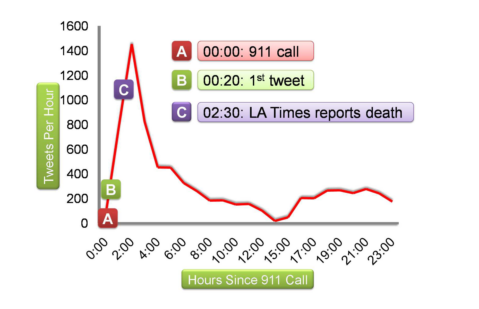
\includegraphics[width=0.8\textwidth]{michael_jackson}
    \caption{Traffic in tweets per hour relating to Michael Jackson’s death by J. Sankaranarayanan \cite{kn:Sankaranarayanan2009}}
    \label{fig:michael_jackson}
\end{figure}

Twitter has not only evolved in terms of usability, but also in the purpose of its use, i.e. Twitter is not only used as personal diary for people but also represents a source of information for reporters and journalists to find potential news about real-time events \cite{kn:Sriram2010}. A good example is given by J. Sankaranarayanan et al. \cite{kn:Sankaranarayanan2009} in the period of Michael Jackson's death. The first tweet about the incident was posted 20 minutes after the call to the 911 emergency service and, nearly, two hours before the first communication on the news as it's possible to verify in the figure \ref{fig:michael_jackson}.

One of the advantages of Twitter compared to other social networks, for example, Facebook, is the easier way to access its users originated data. While Facebook does not provide private information about its users unless there are permissions to do so, or the content shared is present in public pages or groups, Twitter allows the collection of all tweets from channels or directly from people in order to be analysed in any kind of project because the user's accounts are usually public \cite{kn:Musto2015,kn:Stieglitz2013}.

Although this freedom in the collection of data, Twitter has also a an ethical perspective and a regulation must be accomplish by developers or researchers. The TOS (Twitter Terms of Service) was created in order to make known what can be done with the data and protect the users' rights \cite{kn:kelley2013}.

\section{Text Mining}
Text mining is a derived field from Data mining and aims to extract valuable information from unstructured textual data\cite{kn:He2013}. The reason why this technology is nowadays so much explored is because of the massive amount of information that is stored in text documents, such as "text files, HTML files, chat messages and emails" and it's required an automated technique that make possible the identification, extraction, management, integration and the knowledge exploration of information from texts in a efficiently and systematically way \cite{kn:He2013}. On the other hand, the social media applications also have contributed to the growth of text mining usage where companies have seen a potential path to improve their business model and increase the economic value relatively its competitors.

A. Stavrianou et al. \cite{kn:Stavrianou2007} identify text mining as an interdisciplinary field since this technology takes advantages from Data mining techniques and combines several methodologies from similar research areas, such as Categorization, Information Extraction, Information Retrieval, Topic Tracking and Concept Linkage. A common problem related to text mining is its similarity with Information Retrieval and Information Extraction which leads people to a non-differentiation between this technologies. The difference between Information Retrieval and Text mining is established in their final goal, while IR aims to find and retrieve documents that match a certain part of a text or some keywords (e.g. Google Search Engine\footnote{\url{https://google.com}}), TM tries to discovery unknown patterns in texts that can be interpreted and explain some facts or truths contained in the lexical \cite{kn:Stavrianou2007,kn:He2013,kn:Hotho2005}. Regarding the Information Extraction, the differentiation can be seen in the data specificity and structure. IE focus on the extraction of expected information from structured data and precocious relations, while the information returned by TM techniques should be unsuspected and unexpected with the data holding an unstructured format \cite{kn:Stavrianou2007}.

The motivation behind text mining holds on the benefit that other fields of research could take from a use of its techniques. Information Retrieval systems can improve their precision since its basis is the identification of semantic relations. Several areas can explore this methodology to find inconsistencies in relational databases and make the integration, update and querying tasks easier \cite{kn:Stavrianou2007}.

Text mining shares some of the issues presented by the Natural Language Processing field. Once texts are usually performed by humans some associated problems can appear, such as spelling mistakes, wrong phrasal construction, slang among other. Before the "mining" of a text, it's important to apply some pre-processing steps in order eliminating noisy data from the primary analysis process.
A. Stavrianou et al. cite this issues very well in they work and it can be seen in Table \ref{table:textminingissues}.

\begin{table}[]
\centering
\caption{Text Mining Issues by A. Stavrianou \cite{kn:Stavrianou2007}}
\label{table:textminingissues}
\begin{tabular}{ | l | p{7cm} |}
\hline \textbf{Issue}            & \textbf{Details}\\
\hline Stop list                 & Should we take into account stop words?\\ 
\hline Stemming                  & Should we reduce the words to their stems?\\ 
\hline Noisy Data                & Should the text be clear of noisy data?\\ 
\hline Word Sense Disambiguation & Should we clarify the meaning of words in a text?\\ 
\hline Tagging                   & What about data annotation and/or part of speech characteristics?\\ 
\hline Collocations              & What about compound or technical terms?\\ 
\hline Grammar / Syntax          & Should we make a syntatic or grammatical analysis? What about data dependency, anaphoric problems or scope ambiguity?\\ 
\hline Tokenization              & Should we tokenize by words or phrases and if so, how?\\ 
\hline Text Representation       & Which terms are important? Words or phrases? Nouns or adjectives? Which text model should we use? What about word order, context, and background knowledge? \\ 
\hline Automated Learning        & Should we use categorization? Which similarity measures should be applied? \\ \hline
\end{tabular}
\end{table}

The removal of words from the text can sometimes not be desirable because some sentences can lose its information or even leads to a different meaning compared with its original form. The generation of a stop list words should be a supervised task as long as little words could induce distinct results in the text classification \cite{kn:Riloff1995}.

Stemming is a task that depends mostly from the language of the text than its domain \cite{kn:Stavrianou2007} and the main goal of this technique is to reduce a word to its root to help in the calculus of distances between texts or even keywords or phrases.

The noisy data is derived from spelling mistakes, acronyms and abbreviations in texts and to solve this, a conversion of this terms should be done to keep a valid integrity of the data. The most commonly solution approaches involve text edit distances (Levenshtein Distance\footnote{\url{https://en.wikipedia.org/wiki/Levenshtein_distance}}) and phonetic distances measures between known words and the mispelling ones to achieve good corrections \cite{kn:Bontcheva2013} 

Word Sense Disambiguation focus on solving the meaning ambiguity present in words. Other similar field to WSD is Name Entity Disambiguation (NED) where the disambiguation target are named-entities mentions, while WSD focus on common words. WordNet\footnote{\url{https://wordnet.princeton.edu/}} is a resource very used to extinguish this ambiguity \cite{kn:Chang2016}. There are two types of disambiguation, the supervised, where the task is support by a dictionary or a thesaurus \cite{kn:Stavrianou2007}, and the unsupervised one, where the different meanings of a word are unknown and normally learning algorithms with training examples are used to achieve good results in the disambiguation task \cite{kn:Yarowsky1995}.

Tagging can be describe as the process of labeling each term of the text with a part-of-speech tag, i.e. classify each word as a noun, verb, adjective, etc \cite{kn:Hotho2005}. Collacation are very important in text mining, since this task consist in group two or more words to give the correct meaning content in the text. Collacations are usually made before the WSD task since some compound technical terms have different meaning from the individual words which composed it \cite{kn:Stavrianou2007}.

Tokenization serves to pick up all the terms presented in a text document and to achieve this it's necessary the split of the document into a stream of words implying the removal of the punctuation marks and non-text characters \cite{kn:Hotho2005}. some authors also see tokenization as a text representation form since one of the most used models to represent texts is \textit{Bag-of-words} (BoW). This model broke down texts into words and stores it in a vector being also presented the word frequency occurrence in the text. Hence, each word may represent a feature \cite{kn:Sriram2010}. Another commonly used model to represent texts is Vector Space Models that represent all the documents in a multi-dimensional space where documents are converted to vectors and each vector may be seen as a feature. This model provides some advantages since the documents can be compared with each other by performing some specific vector operations \cite{kn:Hotho2005}.

The purpose of this section is to provide the reader the definition of what is text mining, and also the identification of basic operations and steps that are necessary for the preprocessing of this type of unstructured data - texts.

\section{Information Extraction}
Information Extraction is an important field of text mining and its main goal is finding structured information from semi-structured or unstructured texts. This kind of information can range from the identification of entities, such as people, organizations and places names, to a relation between this concepts. In the sentence, \textit{"At 1976, Apple was founded by Steve Jobs and his friends"}, its possible extract information about who were the founders of Apple and what was the year of its foundation. Problems regarding the analysis of the sentence can be located on the words "Apple" and "his", and how could a machine know that "Apple" is a reference of a technological company and not a reference to a fruit, or even, that the word "his" establish a connection between "Steve Jobs" and "friends". The exploration of this kind of information constitutes a potential measure to improve computer systems, such as search engines and database management \cite{kn:Aggarwal2012}.

When the target analysis is social media data, i.e. texts from social networks, the filtering process of the data is a crucial step. It's desirable that only related-topic information should be collected in order to avoid the existence of noisy objects in the data set \cite{kn:Cecilia2016, kn:Saleiro2013}.

Information Extraction presents a set of components that can tackle this problems, such as Named Entity Recognition (NER), Named Entity Disambiguation (NED) and among others.

\subsection{Name Entity Recognition and Name Entity Disambiguation}
NER and NED are two distinct tasks that sometimes could cause some ambiguity in its purpose.

Named Entity Recognition is seen as a sub-task of Information Extraction aiming the correct labeling of words in a text in order to have knowledge of its types. The accuracy retrieve by this task is important when further steps depends on it, e.g. Relation Extraction \cite{kn:Aggarwal2012}. Gazetteers are commonly used in this task since they provide pre-processed lists of organizations, days, places and person names which can be matching against some terms we want to recognize. In some cases, this "tools" are not enough to solve the problem because their domain is very limited and some terms can not exist, implying the use of external knowledge to fill this lack \cite{kn:Ratinov2009}.

There are two main approaches to conduct this task: Ruled-based and Statistical Learning. The Ruled-based approach focus on the definition of a set of features for each token in the text to further comparing the text with a bunch of rules. The rules are composed by patterns that should trigger some labeling action in a sequence of tokens. The definition of this rules usually requires human expertise \cite{kn:Aggarwal2012}. 
The Statistical Learning approach, also known as Statistical Machine Learning, 
treats the text as a sequence of observations which are represented by a vector of features. The final goal of this approach is the assignment of a label $y_{i}$ to each observation $x_{i}$. The mapping process usually follows a BIO notation, firstly introduced to text chunking by \cite{kn:Ramshaw1999}, where the entity name could be at the beginning (B) or inside (I) of the observation and never outside (O). Patawar et al. \cite{kn:Patawar2015} enhance three types of methods to this approach.

Supervised methods, where it's characteristic the existence of a labeled training data set to train a model and then classify a set of test to measure the model performance and accuracy. Hidden Markov Model was used in \cite{kn:Bikel1999} to recognize and classify some text. In \cite{kn:Isozaki2001}, Decision Trees were combined with a simple rule generator to prove that this method could achieve similar results as Maximum-Entropy-based methods used in \cite{kn:Borthwick1999}. Support Vector Machines were used by H. Isozaki et al. \cite{kn:Isozaki2002} where they have proved that SVM models could also achieve good results for NER tasks if some analysis was carefully made in the \textit{kernel functions} and filtering methods were applied, like the removal of useless features.

Semi-supervised methods used different amount of training data, i.e. labeled examples, and test data. The test data is usually a bigger amount facing the training data. The methodology commonly applied to this approach involves the use of "bootstrapping" which is an iterative process of training the model with progressive supervised increases of the training data set until the performance starts to decrease \cite{kn:Irmak2010}.

The last type are the Unsupervised Methods, where a large amount of labeled data is necessary and it's
difficult to have this requirement. This need bases on the huge number of features required to this kind of methods. To fill this lack, a very frequent method used is the clustering where the formation of groups is made using the similarity present in the texts domain \cite{kn:Patawar2015}.

Y. Li et al. \cite{kn:Li2013} define Named Entity Disambiguation as a "process of associating an entity name mentioned in a text to an entry, representing that entity, in a knowledge base". In the last few years, NED has been a target for a considerable number of research projects. The majority methods implemented to tackle this task are focused in three main features. Y. Li et al. \cite{kn:Li2013} enhance \textit{entity popularity} as a statistical one where there is a "assumption that the most prominent entity for a given entity mention is the most probable underlying entity for that mention". At this feature, a link between the term and its Wikipedia page reference is established. The \textit{context similarity} is another feature and aims the complementarity of the \textit{entity popularity} feature. This feature centers on similarity measures between the text in analysis and the content text of the Wikipedia page. Y. Li reveals that this feature is word-dependency since it's necessary that both texts shares identical words in order to produce expected results. \textit{Topical Coherence} is the third feature and solves the emerged problem of the second one. This feature uses the Wikipedia cross-page links mechanism in order to look up for related-topics of other entities and makes a connection with the target entity in the disambiguation problem. Through this process the domain text is expanded, decreasing the word-dependency problem appeared in the second feature.

D. Spina et al. \cite{Spina2013} present two different approaches to solve the problem of ambiguity presented in texts. The first one is \textit{entity linking} and consists in the establishment of an association between the mention in the text and a entity present in a Knowledge Base. Three steps are needed to perform the linking of the entity name to the knowledge base:

\begin{itemize}
\item \textbf{Query Expansion:} Mining the Wikipedia structure and solving co-references in the document in order to enrich the query;
\item \textbf{Candidate Generation:} Construction of a list of candidate entities from the knowledge base according to the information presented in the query;
\item \textbf{Candidate Ranking:} It is the phase in which is computed some similarity measures between the query and the entities, in order to rank the candidates and select the best one.
\end{itemize}

Another approach to tackle this problem of disambiguation of entities presented by D. Spina et al. \cite{Spina2013} is the \textit{document enrichment by linking to Wikipedia Articles}. Similar to the \textit{entity linking}, this approach is also composed by three different steps and takes advantages from text representation models, such as Bag-of-words or Vector Space Models, for example.

\begin{itemize}
\item \textbf{Mention or surface form representation:} There a context definition of the target mention to disambiguate. Text representation models are build with all set of entities that are ambiguous and the unambiguous ones which are already resolved with linking to Wikipedia pages.  
\item \textbf{Candidates entities retrieval and representation:} All the candidate entities referenced by the knowledge base (e.g. Wikipedia or Freebase) and the content on the page are converted to text representation models. After this, there is extraction of some features that can range from page categories of the candidate entities or even syntactic features.
\item \textbf{Best candidate selection:} The computing of similarity and distance functions between the two text representation models, produced in the two previous steps, is made to select the best candidate. 
\end{itemize}

Some works related to NED were made in the context of micro-blogging services, such as Twitter.

At 2010, Ferragina et al. \cite{kn:Ferragina2010} developed a system capable of identity entities in short texts as, for example, tweets. Their system take advantage of the hyperlink mechanism of Wikipedia, extracting related links between pages and the anchors texts in the links. By detecting some senses present in the anchors, they try to disambiguate the ambiguous ones through a collective agreement function, i.e. a voting classification. They used the unambiguous senses to boost the selection of the ambiguous ones and have trying some pruning in the anchors set to improve the performance of the system.

Meji et al. \cite{kn:Meij2012}, similar to Ferragina et al., also explored anchors texts in Wikipedia articles. The authors have used a supervised machine learning approach to conceive a list of candidates to disambiguate each mention present in their tweets. Their strategy focus on the identification of some patterns in each tweet, such as n-grams, to further matching it with the anchor texts of the Wikipedia articles, taking also in account the hyperlink mechanism of this Knowledge Base.

Considering this works it's possible conclude that Wikipedia is a potential source to explore in order to solve mentions of entities that could lead to a ambiguous problem. 

\subsection{Content Filtering}
The content filtering is one of the most important tasks to analyze micro-blog data (e.g. Twitter). The main goal of content filtering is the classification of Twitter posts which contains an entity name, assuming the existence of a relation between the name and the content in order to erase ambiguity in the dataset \cite{kn:spina2014}. Recently, some contests related with Online Reputation Monitoring (ORM) have explored this task of filtering content. The WePS-3 \footnote{\url{http://nlp.uned.es/weps/}} and the RepLab 2012 tackle unknown-entity scenario approaches, while the RepLab 2013 \footnote{\url{http://nlp.uned.es/replab2013/}} focus on the known-entity scenario approach.

In the WePS-3, the LSIR \cite{kn:Yerva2010} research group has build a system where a profile identify each of the companies mention. The Wordnet \footnote{\url{https://wordnet.princeton.edu/}} and the company web-page were used to extract a bunch of keywords related with the company. Combining this previously set of keywords with some manually defined they have created the profiles to the companies in analyse. They used this profiles to extract specific features from "tweets" and added to a set where there already was some generic features. This information was further used to classify the tweets with "related/unrelated" labels.

Regarding the ITC-UT \cite{kn:Yoshida2010} research group, they have, firstly, made a prediction of the company name class according to the related-tweet ratio. After this step, a distinct heuristic was found to each of the classes, using basically part-of-speech tagging and the named entity label of the company. Their approach was a two-step classification task.

SINAN \cite{kn:Cumbreras2010} system used an approach of ruled based heuristics, specially the existence of the entity name both on tweets and external resources, such as Wikipedia, DBPedia \footnote{\url{http://wiki.dbpedia.org/}} and the company web-page.

The RepLab 2012 follows an identically problem as the WePS-3, the unknown-entity scenario. Some research teams follow the same approach as S. Yerva et al. \cite{kn:Yerva2010} where the use of profiles describing each company mention to correctly filter the content. DAEDALUS \cite{kn:villena2012} and OXYME \cite{kn:kaptein2012} tackle a manually exploration, such as the development of dictionaries and rules sets to the detection and the classification task, and the selection of feedback terms about the entities, respectively. The automatically methods were explored mainly with external resources. CIRGDISCO \cite{kn:Qureshi2015} and ILPS \cite{kn:peetz2012} used the Wikipedia, while BMEDIA \cite{kn:Chenlo2012} combined it with Freebase to extract related and unrelated concepts. CIRGDISCO proposed a two-step algorithm to solve the filtering task. The first step involves the extraction of the entity related-terms from the Wikipedia and further calculus of the IDF (Inverse Document Frequency) score for each term founded. The second step focus on the idea of concept term score propagation, i.e. to propagate the labels of the high-precision classified tweets to the remaining, in order to increase the recall measure. ILPS tackle the filtering task by using semanticising, where two probabilities are verified: Link Probability and Commonness. The first one represents the probability that an n-gram is linked to an Wikipedia page, while the second is the probability of an n-gram is linked to a certain concept. The ILPS group also used list aggregation and disambiguation techniques to carry out this task.

At RepLab 2013, the filtering task was in a known-entity scenario where the data provided to the groups consists of a collection of tweets about 61 entity names in two distinct languages, English and Spanish. Saleiro et al. \cite{kn:Saleiro2013} have devolved POPSTAR which was the system that, using a supervised learning, has obtained the best results classifying the tweets as related or non-related with the entities. Their group has explored internal features (RepLab Metadata, probabilities in the text, keyword similarities) and external features, such as Web Similarity (between tweet text and the Wikipedia page text) and Freebase scores relatively to the position of the target entity in the retrieved list.

The second best score in the filtering task at RepLab 2013 was obtained by V. Hangya et al. \cite{kn:hangya2013} where their system made usage of text normalization methods, combining the textual features with topic distribution features retrieved by a LDA (Latent Dirichlet Allocation) model. The resulting features were further used in a maximum entropy classifier to perform the filtering task. The LIA \cite{kn:Cossu2013} group has used k-Nearest-Neighbour (kNN) algorithm with a set of discriminant features based on similarity measures. They have used Bag-of-Words representation, combining TF-IDF (Term Frequency-Inverse Document Frequency) with Gini purity criteria, for the tweets collection and calculated the Jacard similarity measure.

This kind of methodologies will be a huge step to validate our dataset since it's important to have only related-topic tweets to analyze the people's feelings, opinions about a correct entity instead unrelated ones.

\subsection{Topic Modeling} \label{subsec:topicmodeling}
The emergence of topic modeling techniques was due to the people's chase of a better understanding of the available information in document corpora. Topic models provide the discovery of certain patterns in a collection of texts and enhance specific words/terms that have a direct relation to the content information \cite{kn:Mehrotra2013}. There are many studies that were conducted in order to prove that is possible to extract coherent topics from micro-blogging data using the LDA (Latent Dirichlet Allocation) model \cite{kn:Mehrotra2013, kn:Hong2010, kn:Zhao2011}. LDA models are difficult to apply to micro-blogging texts because of the characteristics present in this kind of text: short, mixture of contextual clues (URLs, tags, name mentions with the '@'), informal language with many misspelling, acronyms and abbreviations \cite{kn:Mehrotra2013}. L. Hong et al. \cite{kn:Hong2010} describe Latent Dirichlet Allocation as "an unsupervised machine learning technique which identifies latent topic information in large document collections". This technique uses "bag-of-words" to each document which  are represented by a probability distribution over some topics, and each topic is, in turn, represented by a probability distribution over a number of words.

R. Mehrotra et al. \cite{kn:Mehrotra2013} have explored the improvement of the standard LDA model using several pooling schemes of tweets, i.e. aggregating tweets by some characteristics present in its content. Their polling schemes characterization range from basic scheme: where each tweet is treated as a single document; author-wise pooling: aggregating the tweets according its author; burst-score wise pooling: tweets are aggregated by the scores obtained from the execution of a burst detection algorithm; temporal pooling: pools are formed by tweets posted at the same hour; \textit{hashtag}-based polling: the tweets are grouped according to its \textit{hashtag} (\#) reference, and if there are more than one reference then the tweet is added to each of the groups. The authors evaluate the resulting clusters through some metrics, such as the \textit{purity}: verifying the average of the corrected labeled tweets inside the clustering; \textit{normalized mutual information} (NMI): its the calculus of the matching results between the clustering and the category labels; and finally the \textit{pointwise mutual information} (PMI): measure of the statistical independence between two words regarding the close proximity. Their approaches also were studied combining similarity tag assignment (TF and TF-IDF) and the best presented results were performed by \textit{hashtag}-based polling with TF-similarity tag assignment regarding the purity and the NMI metrics, while the best PMI metric was obtained by the simple \textit{hashtag}-based polling method.

L. Hong et al. \cite{kn:Hong2010} also explored the LDA models through a set of schemes formed by them. Their schemes diverge between user-based and term-based groups, where the user-based are agglomerations of messages from the same user while the term-based groups are formed by messages that have the same term in the content. In their approach they have also used Author-Topic Model which is an extension of the LDA model but the main difference is that in the LDA, each document is associated with a multinomial distribution over T topics while in the AT model the association is made to the author instead the document. They used JS Divergence to study the similarity between the performed schemes. The main goal of their work was not the topic modeling but they proved that this sub-task can improve performances of classification, namely when the messages are group by the same user.

W. Zhao et al. \cite{kn:Zhao2011} proposed another extension of the LDA model and named it Twitter-LDA \footnote{\url{https://github.com/minghui/Twitter-LDA}}. Their model follows the idea that each tweet is about some topic, so instead of grouping the tweets into schemes and than extract some topic, they tackle each tweet as a singular problem and extract the target of the content. In their work, the evaluation of the model was made by comparing its effectiveness against the standard LDA model and the Author-topic model. The Twitter-LDA results, obtained from a small set of topics in a preliminary test, have surpass the performance of the others models (standard LDA and Author-topic models).

The last model should be a good start to face the problem of topic modeling in our work, since it's open-source tool and it's available in GitHub.

\section{Sentiment Analysis}
Sentiment Analysis is a task of NLP (Natural Language Processing) and aims the finding of the polarity in opinions, sentiments of people about a specific topic contained in a document or even the overall sentiment present in it. Research done in this area has grown at an impressive pace and this is due to the value that this type of analysis can provide to the business world. "Marketing managers, PR firms, campaign managers, politicians, and even equity investors and online shoppers are the direct beneficiaries of sentiment analysis technology" since the retrieved information can favor and make easier the decision-making process \cite{kn:Feldman:2013}. This task is composed by several distinct problems and there are two main approaches to tackle it: supervised \cite{kn:Saleiro2016, kn:Kouloumpis2011} and unsupervised \cite{kn:Musto2015, kn:Allisio2013}. Feldman in their work \cite{kn:Feldman:2013} enhaces the several types of problems found in the sentiment analysis task. One of them, the document-level sentiment analysis focus on the determination of the sentiment polarity of opinions expressed by the author in his document. Another problem that is widely explored is the sentence-level sentiment analysis which is a deeper version of the previous. A document may have multiple opinions about a specific entity and in order to extract the polarity value about it, a phrase-level split is required. Some countermeasures must be taken into account in the polarization of phrases since the sarcasm component can be present in the content and it's very difficult to treat correctly this. There is another problem in this field named aspect-based sentiment analysis where the sentiment polarity should be directed to the aspects/topics contained in the document. In the following subsections a deep description and studied solution of this problem will be presented.

\subsection{Lexicon-based vs Machine-learning based} \label{subsec:lexi_mach}
Sentiment analysis in Twitter can be divided in three different approaches relatively to the sentiment classification: lexicon-based, machine-learning based or even a hybrid approach between the previous two. In the first place it's necessary to talk about what features are relevant or not in order to tackle this problem. Aggarwal et al. \cite{kn:Aggarwal2012} in his work refer some of the common features used in this problem:

\begin{itemize}
\item \textbf{\textit{Term presence and frequency:}} groups of words, named \textit{n-grams}, and the frequency they occur in the document;
\item \textbf{\textit{POS Tag}}: the existence of adjectives can be relevant indicators to determine the opinion polarization;
\item \textbf{\textit{Opinion words and phrases:}} words that usually transmits some polarity, such as \textit{good and bad}, or even whole phrases that don't have this type of words, e.g. "cost me an arm and a leg";
\item \textbf{\textit{Negation}}: the existence of negative words that may change the opinion orientation, such as "I don't like apples" which means the same as \textit{hate}. 
\end{itemize}

After the features engineering process, it may be necessary to select only a few ones to apply in the classification task. W. Medhat et al. \cite{kn:Medhat2014} mentioned in their work some of the most used methods in this particular step:

\begin{itemize}
\item \textbf{\textit{Lexicon-based:}} It's necessary human annotation. Starts with a small set of seed words and then a bootstrapping methodology is applied to expand the lexicon domain through the discovery of synonyms in external resources;
\item \textbf{\textit{Point-wise Mutual Information}}: It's a statistical method where the co-occurrence level between a given word $w$ and a class $c$ is computed in order to see if a feature is or not correlated with the class. The formula of calculus is given in the equation \ref{eq:pmi},

\begin{equation} \label{eq:pmi}
 M_c(w) = \log(\frac{F(w).p_c(w)}{F(w).P_c}) = \log(\frac{p_c(w)}{P_c})
\end{equation}

where $F(w).P_c$ is the expected co-occurrence level and $F(w).p_c(w)$ is the true value of the co-occurrence.

\item \textbf{\textit{Chi-square}}: It's another statistical method used to measure the correlation between the features and the classes \ref{eq:chi_square},

\begin{equation} \label{eq:chi_square}
X_c^2 = \frac{n.F(w)^2.(p_c(w)-P_c)^2}{F(w).(1-F(w)).P_c.(1-P_c)}
\end{equation}

where $n$ is the total number of documents that composed the collection, $p_c(w)$ represents the conditional probability of class $c$ in the documents containing the word $w$, $P_c$ are the fraction of documents that contain the class $c$ and $F(w)$ are the documents fraction that contain the word $w$.

\item \textbf{\textit{Latent Semantic Indexing}}: It's an unsupervised method that aims the reduction of the original set of features into a new ones through transformation techniques like PCA (Principal Component Analysis)
\end{itemize}

After the conclusion of this step of features selection, the sentiment classification is conducted and there are a very high number of techniques that can be applied.

A. Giachanou et al. \cite{kn:Giachanou2016} divided the \textbf{machine-learning approaches} into three different categories: supervised learning, the classifiers ensembles and deep learning.

Supervised learning methods focuses on the training of classification models with a manually labeled dataset, also named training dataset,  and various features extracted from the Twitter messages in order to submit a test dataset under the model and have an automatic prediction regarding the polarity of the sentiment (positive, negative or neutral) in the message. There are many types of classifiers, such as Naïve Bayes (NB), Maximum Entropy (ME), Support Vector Machines (SVM), Logistic Regression (LR), Random Forest (RF) or even Conditional Random Fields (CRF). In the last few years, many studies of Twitter sentiment analysis using supervised learning were conducted. At 2009, Go et al. \cite{kn:Go2009} tackle a problem of binary classification about Twitter sentiment analysis using SVM, NB and ME algorithms and distant supervision to produce their classifier models. Their dataset was composed by 1.6 million twitter messages and they don't have the problem of imbalanced classes. As features they used POS tags, unigrams and bigrams and they also have in consideration the existence of negation in the messages. The best performance they have obtained was with the Naïve Bayes model and as final conclusions they said that using POS tags as feature doesn't improve the final accuracy. 
Hamdan et al. \cite{kn:hamdan2013} made some experiments using SVM and NB models in Twitter messages but their set of features was different from the previous work mentioned. The authors use DBPedia to extract concepts, WordNet to extract adjectives, Senti-WordNet to extract the sentiment score of some words and also have in consideration the existence of emoticons in the message. As final results they concluded that the SVM model performance surpasses the NB model between 2\%-4\%, and for that they have used the harmonic mean F-measure as evaluation metric. 
Saleiro et al. \cite{kn:Saleiro2016} work with Twitter messages to study the political opinions about the five political leaders during the Portuguese bailout between 2011 and 2014. The features they have used were composed by sentiment aggregate functions applying them to a non-linear regression model using the Random Forests algorithm and to a linear regression model using the Ordinary Least Squares (OLS) algorithm. The authors have grouped the dataset per month in order to see what was the monthly variation. In the validation process, a 10-fold cross validation was used and regarding to the evaluation metric they explore the Mean Absolute Error (MAE).

The Classifiers Ensembles approach is based on the combination of several classifiers to improve the performance of the classification task. The workflow of this approach can be verified in the figure \ref{fig:ensemble-classifiers}. da Silva et al. \cite{kn:daSilva2014} have explored the sentiment analysis in Twitter using a combination between Random Forests, Support Vector Machines, Multinomial Naïve Bayes and Linear Regression. The final classification decision in this kind of approach is usually made by majority voting between the models. In their work, da Silva et al. decided to calculate the average between all classification probabilities given by the models and applied that resulting value to the decision task.

\begin{figure}
  \caption{The workflow of the classifiers ensembles by da Silva et al. \cite{kn:daSilva2014}}
  \centering
    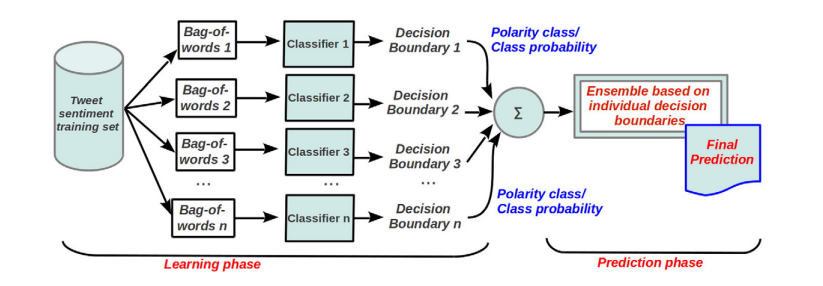
\includegraphics[width=1\textwidth]{ensemble-classifiers}
    \label{fig:ensemble-classifiers}
\end{figure}

Hassan et al. \cite{kn:Hassan2013} have explored a different approach regarding the classifiers ensemble. They proposed a framework that was composed by seven different classification algorithms and used bootstrapping to the sample input in order to provide a small portion to each model. Their set of features had several types: semantic, POS tags, sentiment scores (SentiWordNet) and n-grams. Information Gain criteria was used to the feature selection process. By using bootstrapping in their framework, the problem of imbalance classes was reduced which could be a great advantage to explore in our approach.

Deep learning (DL) is the third and last method in the supervised learning approaches. DL is a recent field in the area of Machine Learning which may imply a scarcity in its addressed use to the sentiment analysis on Twitter \cite{kn:Giachanou2016}.
The studies conducted in this method took advantages from the SemEval-2013 and SemEval-2014 datasets. Tang et al. \cite{kn:tang2014learning} developed three different neural networks models to learn sentiment specific word embeddings (SSWE). The results provide by the models were later used as features to classify the polarity of sentiment in the dataset messages. The authors have combined the obtained features with others like sentiment lexicons \cite{kn:tang2014learning}, emoticons, negation, n-grams, punctuation, clusters, etc \cite{kn:tang2014coooolll}. The evaluation metric used to measure the performance of their classification models was the F-measure. The best result obtained to the SemEval-2013 dataset was 86.58\% while for the SemEval-2014 dataset was 87.61\%.

There are a high diversity in the methods to apply supervised learning, i.e. application of machine-learning algorithms, to automatic classify the sentiment polarity either on tweets or opinion reviews. The problem in its use focuses on the features engineering which is a hard task and the learning algorithms effectiveness depends on its selection. The bad choice of some features may cause that the final results obtained are not the most desirables.

Contrary to the machine-learning approaches, the \textbf{lexicon-based approaches} doesn't depend on training data and features to classify the sentiment as positive, negative or neutral. In this approach the final sentiment classification is given by measuring the sentiment score of each term using external resources, such as dictionaries with a large number of previously evaluated terms (SentiWordNet \footnote{\url{http://sentiwordnet.isti.cnr.it/}}, SenticNet \footnote{\url{http://sentic.net/}}, LIWC \footnote{\url{http://liwc.wpengine.com/}}). At 2010, Thelwall et al. \cite{kn:Thelwall:2010} developed a lexicon-based algorithm, named SentiStrength \footnote{\url{http://sentistrength.wlv.ac.uk/}}, capable of detecting the sentiment value in messages that usually have informal language, such as tweets. The algorithm have access to 298 positive terms and 465 negatives and to a list of emoticons, negations and booster words to increase or decrease the sentiment value of derived words. The authors have compared their algorithm with machine-learning approaches and the results were very interesting since in terms of accuracy as evaluation metric, SentiStrength has surpass the others.

C. Musto et al. \cite{kn:Musto2015} have developed a domain-agnostic framework to produce some social media analytics regarding some events that happen in Italy in the last years. They evaluate the sentiment present in each tweet using lexicon-based approaches. The external resources used were SenticNet and SentiWordNet. The authors have split each tweet message by cues, such as punctuations and conjunctions, creating two or more micro-phrases. After this step, each micro-phrase is classified according the scores of the terms present in the resources. The sentiment polarity of the original message is obtained by summing its related micro-phrases. They also studied an emphasized approach where the Part-of-speech (POS) category of each term has a weight. Adverbs, verbs and adjectives received a value greater than 1, while for the remaining categories the value was 1.

L. Allisio et al. \cite{kn:Allisio2013} proposed a framework, named Felicittà, in order to measure the hapiness level in the Italian territory. The study was made on geotagged tweets and it was used the resources MultiWordNet \footnote{\url{http://multiwordnet.fbk.eu/english/home.php}} and WordNet-Affect \footnote{\url{http://wndomains.fbk.eu/wnaffect.html}}. All the emoticons presented in the tweets were replaced by its meaningful words. The approach used by the authors consists in for each tweet term, a search is computed in the MultiwordNet dictionary to find all the meanings the word can have. After this step, each meaning found is associated with the sentiment score present in the WordNet-Affect corpus. The sum of all meanings is calculated, assigning a value of -1, 0 or 1 to the term. The tweet final classification is done by calculating the mean polarity of all terms and comparing with a heuristic constant defined by the authors.

The lexicon-based approaches are simpler to implement compared with the machine-learning approaches. They also presented disadvantages as the need of a continuously update of the word lists (lexicon sentiment dictionaries) because the conversation themes on Twitter are always changing which may result in the absence of words in the lists, and consequently their scores \cite{kn:Giachanou2016}. For this reason, the missing words are not considerate to the sentiment polarity classification and the results may not be so reliables.

The last approach for sentiment analysis is a mixture of the two previously presented, a \textbf{hybrid approach}. This kind of approach was explored by Ghiassi et al. \cite{kn:Ghiassi2013} where they used machine-learning algorithms (SVM and Dynamic Artificial Neural Networks - DAN2) with a n-gram analysis. The collection of tweets was about Justin Bieber and as features to the classifiers, the authors choose emoticons, tweets that have positive and negative words, e.g. \textit{happy or sad}, and also synonyms of this words. The model DAN2 proved be the best in the classification task.
A. Kumar et al. \cite{kn:kumar2012} mixed a log-linear regression model with lexicon-based methods. Firstly, they have made pre-processing to the tweets collection by removing the URL references, replacing emoticons with their score value, calculate the percentage of caps in the message and also the sentiment orientation of the adjectives, verbs and adverbs. The overall sentiment of the tweet message was computed by the linear equation of the model, which was enough to prove the efficiency of the approach explored by the author relatively to the polarity of a tweet.

The main advantage of the hybrid approach establishes in the no need to manually classify the dataset for its use in machine learning methods. By applying lexicon-based methods we can have a labeled dataset ready to be use in ML classifiers. A disadvantage on this approach is high computational power need to bear out both approaches at the same time \cite{kn:Giachanou2016}.

\subsection{Aspect-based Sentiment Analysis}
Aspect-based sentiment analysis (ABSA) is the most difficult problem to solve regarding the field of sentiment analysis. This approach focuses on the recognition of aspects in the messages and consequently on their sentiment polarity classification.

In particular to the aspect extraction, an overview was already done in the subsection \ref{subsec:topicmodeling} where the topic-based approach was mentioned and described using the LDA model as the most used model. There are three more approaches that we can follow to discover relevant aspects in a document: frequency-based \cite{kn:hu2004}, ruled-based \cite{kn:Gindl2013} and supervised learning \cite{kn:Jakob, kn:Jin2009}.

The frequency-based approach focus on finding some nouns or noun phrases from a large corpus using the occurrence frequency as the main requirement. M. Hu et al. \cite{kn:hu2004} used this approach in order to summarize some customer reviews regarding a set of products. They used POS tagging to found nouns and noun phrases present in the document and association mining to find frequent itemsets because the features that composed the itemset are usually product features. After this step, they submitted the features set to a pruning section in order to remove the meaningless ones.

In the ruled-based approach, S. Gindl et al. \cite{kn:Gindl2013} have made a study in order to prove that it's possible identify and extract aspects in sentences by propagating the sentiment charge to noun targets following a set of defined rules. They have verified a problem when the sentiment and the aspect mention are in different sentences. Simple propagation rules are not enough to found the aspects. To overcome this, they have defined another rule where if a sentence starts with a pronoun, the target aspect is probably the last noun identify in the previous sentence.

Supervised learning approaches are based in sequential learning methods, such as Conditional Random Fields (CRF) and Hidden Markov Models (HMM). The mentioned methods are similar because both of them attempt to discover patterns relative to an input data set. These types of methods are often used in the aspect extraction task of opinion mining. N. Jakob et al. \cite{kn:Jakob} has built a classification model using the CRF algorithm in order to enhance the target of each opinion in the reviews. The domain of their dataset was constituted by four independently categories: movies, web-services, cars and cameras. Since the approach taken by the authors was through machine learning classifiers, they had the need of establishing a set of features to train the model. The features used for the classification vary from the string of each token, the POS tag for each token, the level of dependency between each token and the opinion expressed as well as its word distance, and, finally, the last feature is the opinion sentence itself to allow the CRF algorithm the ability of distinguish when a token is present or not in a sentence that is an opinion. Regarding the system validation, the authors applied also a 10-fold cross-validation to see if the model performance improves or not. As performance metrics to evaluate the system, they used the precision (Equation \ref{eq:precision}),

\begin{equation} \label{eq:precision}
\frac{TP}{TP+FP}
\end{equation}

the recall (Equation \ref{eq:recall})

\begin{equation} \label{eq:recall}
\frac{TP}{TP+FN}
\end{equation}

and the F-measure (Equation \ref{eq:f-measure}) that is the harmonic mean between the previous two metrics.

\begin{equation} \label{eq:f-measure}
2.\frac{precision.recall}{precision+recall}
\end{equation}

W. Jin et al. \cite{kn:Jin2009} also worked under the opinion reviews and tried to find relevant opinion targets in the content. They have developed a novel framework based on machine learning techniques. The framework, named OpinionMiner, appeals to a classification model with the HHM algorithm and to a bootstrapping approach in the training step. The bootstrapping divides the main process of training in two sub-process as well as the training dataset into little portions in a randomly way. Each sub-process has his own HHM model and after its training step, the main process only selects the objects which their label is agreed by both classifiers. The bootstrapping process is repeated until no more targets in the objects can be discovered.

Regarding the polarity sentiment classification, the majority of the works studied appeals to one of the approaches described in the section \ref{subsec:lexi_mach}.

\section{Conclusion}

This chapter had the objective of review some basic concepts that may be relevant to contextualize the reader about the problem of performing analysis in social media streams, e.g. Twitter messages. Hence, the literature studied was divided in several points in order to have a overview about what is already done and what are the approaches that some author proposed to tackle each of the sub-problems that composed the main problem in this dissertation work.
After a careful research, it was possible to identify that there are a great diversity of approaches to each sub-problem, whether it be disambiguation, filtering, topic detection or even sentiment analysis.

An important point identified in the literature was the few works done using deep learning to take the problem of sentiment analysis with supervised leaning approaches, since its applicability in the artificial intelligent field has grown at an exponential level in the recent years.

Regardless the task that the authors dealt with, it was possible to identify that the features engineering process and its selection, when their proposed solution used classifier models, is similar. This may be an advantage to the development of the different modules that composed the proposed framework in this dissertation work.

The framework modules will also have classifier models, so the evaluation and validation of it is important. The literature review shows a large set of evaluation metrics to do this step.

In short, it is expected from the reader that this review to the State-of-the-Art has provided a coherent understanding regarding the study of different real scenarios using the social media streams as source of information.

\chapter{Framework} \label{chap:framework}

\minitoc \mtcskip \noindent

In this chapter it is described the details and specificities of the framework proposed in this dissertation. First, we enunciate the necessary requirements to fulfill and achieve the mentioned development. Moreover, it is present the framework architecture design, as well as it inner pipeline. The modules that constitutes such architecture are described afterwards as so the required methodologies and algorithms incorporated in each of its tasks. Finally but not least, we mentioned and explained the different data visualizations available in the framework.

\section{Requirements}\label{sec:requirements}

The development of frameworks to the domain of \textit{smart cities} and intelligent transportation systems using human-generated content (e.g. text messages) is a laborious and time-consuming process. The source of the data to fed such system is one of the biggest challenges in this kind of developments, ranging from social media, smart phones and urban sensors. In this dissertation we tackle the problem of exploring social media data since this kind of data have, recently, been seen as a new opportunity and source to mine valuable information to the cities services and corresponding responsible entities~\cite{kn:Musto2015}.

Social media data are mostly represented by text messages being necessary the application of Natural Language Processing (NLP) methodologies in order to extract information from its content. Such methodologies are usually complex and composed by several different steps (e.g. some related to the syntax of the sentences while others are related to the semantics of its content) before the achievement of the desired results. Social Media streams are no exception, indeed, the analysis of such texts is even more complex since messages are usually short and present lots of informal characteristics.

A framework for the domain of social media content requires, in the first place, a data collection module. Depending on the social network, the data collection module can have different heuristics with respect to the data retrieving. Here, the choice of such heuristics is important and needs to be made according the final users expectations, or at least, according the framework final use case. Towards the application of NLP techniques, a module in charge of preprocessing tasks is required. The main purpose of this module establishes in the performance and robustness of the results obtained by the previously mentioned techniques. NLP techniques can provide different types of information, however in this dissertation the focus is on the classification of travel-related tweets and characterization of the topic associated with a tweet. Each technique is represented as an independent module whose belongs to the boundary of text analytics. This framework needs to also be capable of processing information regarding the creation date of a tweet, \textit{metadata} and geographic distribution associated to it. For the fast retrieving of this informations to the data visualization view, some aggregations need to be made. This requirement is due to one of the big data demands, the instantly availability of the results. Such demand is important for the framework end-users since it helps in the entities' decision-making process making easier and faster the improvement of its services.

The construction of this complex system requires careful planning since there are dependency between a task and the one that follows it, at least with respect to the filtering and preprocessing of data. Adaptability to different languages is considered and further addiction of new ones may be possible. For the same reason, but this time regarding new functionalities, the framework needs to follow a modular architecture allowing new text analysis layers as well as other type of data visualizations. The domain of \textit{smart cities} is vast in terms of the indicators and fields constituting it and due to that, the final architecture may be designed in a way that allows configuration about the user's field of interest if this do not wishes analytics visualization from all fields.

\section{Architecture Overview}\label{sec:architecture}

The framework proposed in this dissertation is divided into six different modules: (1) collection; (2) filtering; (3) preprocessing; (4) text analytics; (5) aggregation and (6) data visualization.

The current collection module is currently implemented to collect geo-location tweets from a specific bounding-box, however if the user demands, multiple locations can be explored at the same time. Other collection heuristics are also available, such as the keyword-search and users following. Depending on the target scenario and analytics to be explored, these two heuristics will need to be added in the module. This detail was considered during implementation period and flexibility was assure into the module composition.

Filtering tasks are directly related to \texttt{locations} heuristic of the collection module. Since this framework is designed to analyse cities or specific regions/zones of it, it is necessary guarantee if a tweet is actually inside of the searching bounding-box in order to do not induce information in the analysis from places far away of the target location. If other heuristics will be implemented, the filtering module can be configured to support other specific filtering operations.

The preprocessing module is a module that has into consideration the future task in the framework. Having this considered, we implemented a segmented pipeline allowing the user a definition of the desired tasks he wants to analyse in the text messages since different text analysis may have different operation in the preprocessing routine. Methods implemented here are carefully described in Section~\ref{sec:data_preprocessing}.

Text analytics module is composed by two different sub-modules, both of them focusing in a specific text analysis method. Travel-related classification of tweets for two different speaking languages is available since one of the final goals regarding domain-agnostic framework is its adaptability into different scenarios and the language of texts constitutes one of them. Topic Modelling sub-module is available as a text analytics method provided by the framework. We trained a model over a sample of tweets and characterize each topic generated in order instantly characterize future tweets by only being necessary passing it over the transformation process to have their topic identified.
In terms of generalization, the main module, text analytics module, was construct following adaptability and flexibility approaches to, in the future, new analysis be integrated.

By adding new functionalities, new aggregations are required in order to present the specific-task final results to the end-user. The aggregation module is structured into integrative methods facilitating future extensions or updates on it. Last but not least, aggregation results are communicated to the visualization module, where, similar to other modules, it is possible the inclusion of new data visualization charts, according to the new integrated functionalities.

\begin{figure}[htbp]
	\centering
	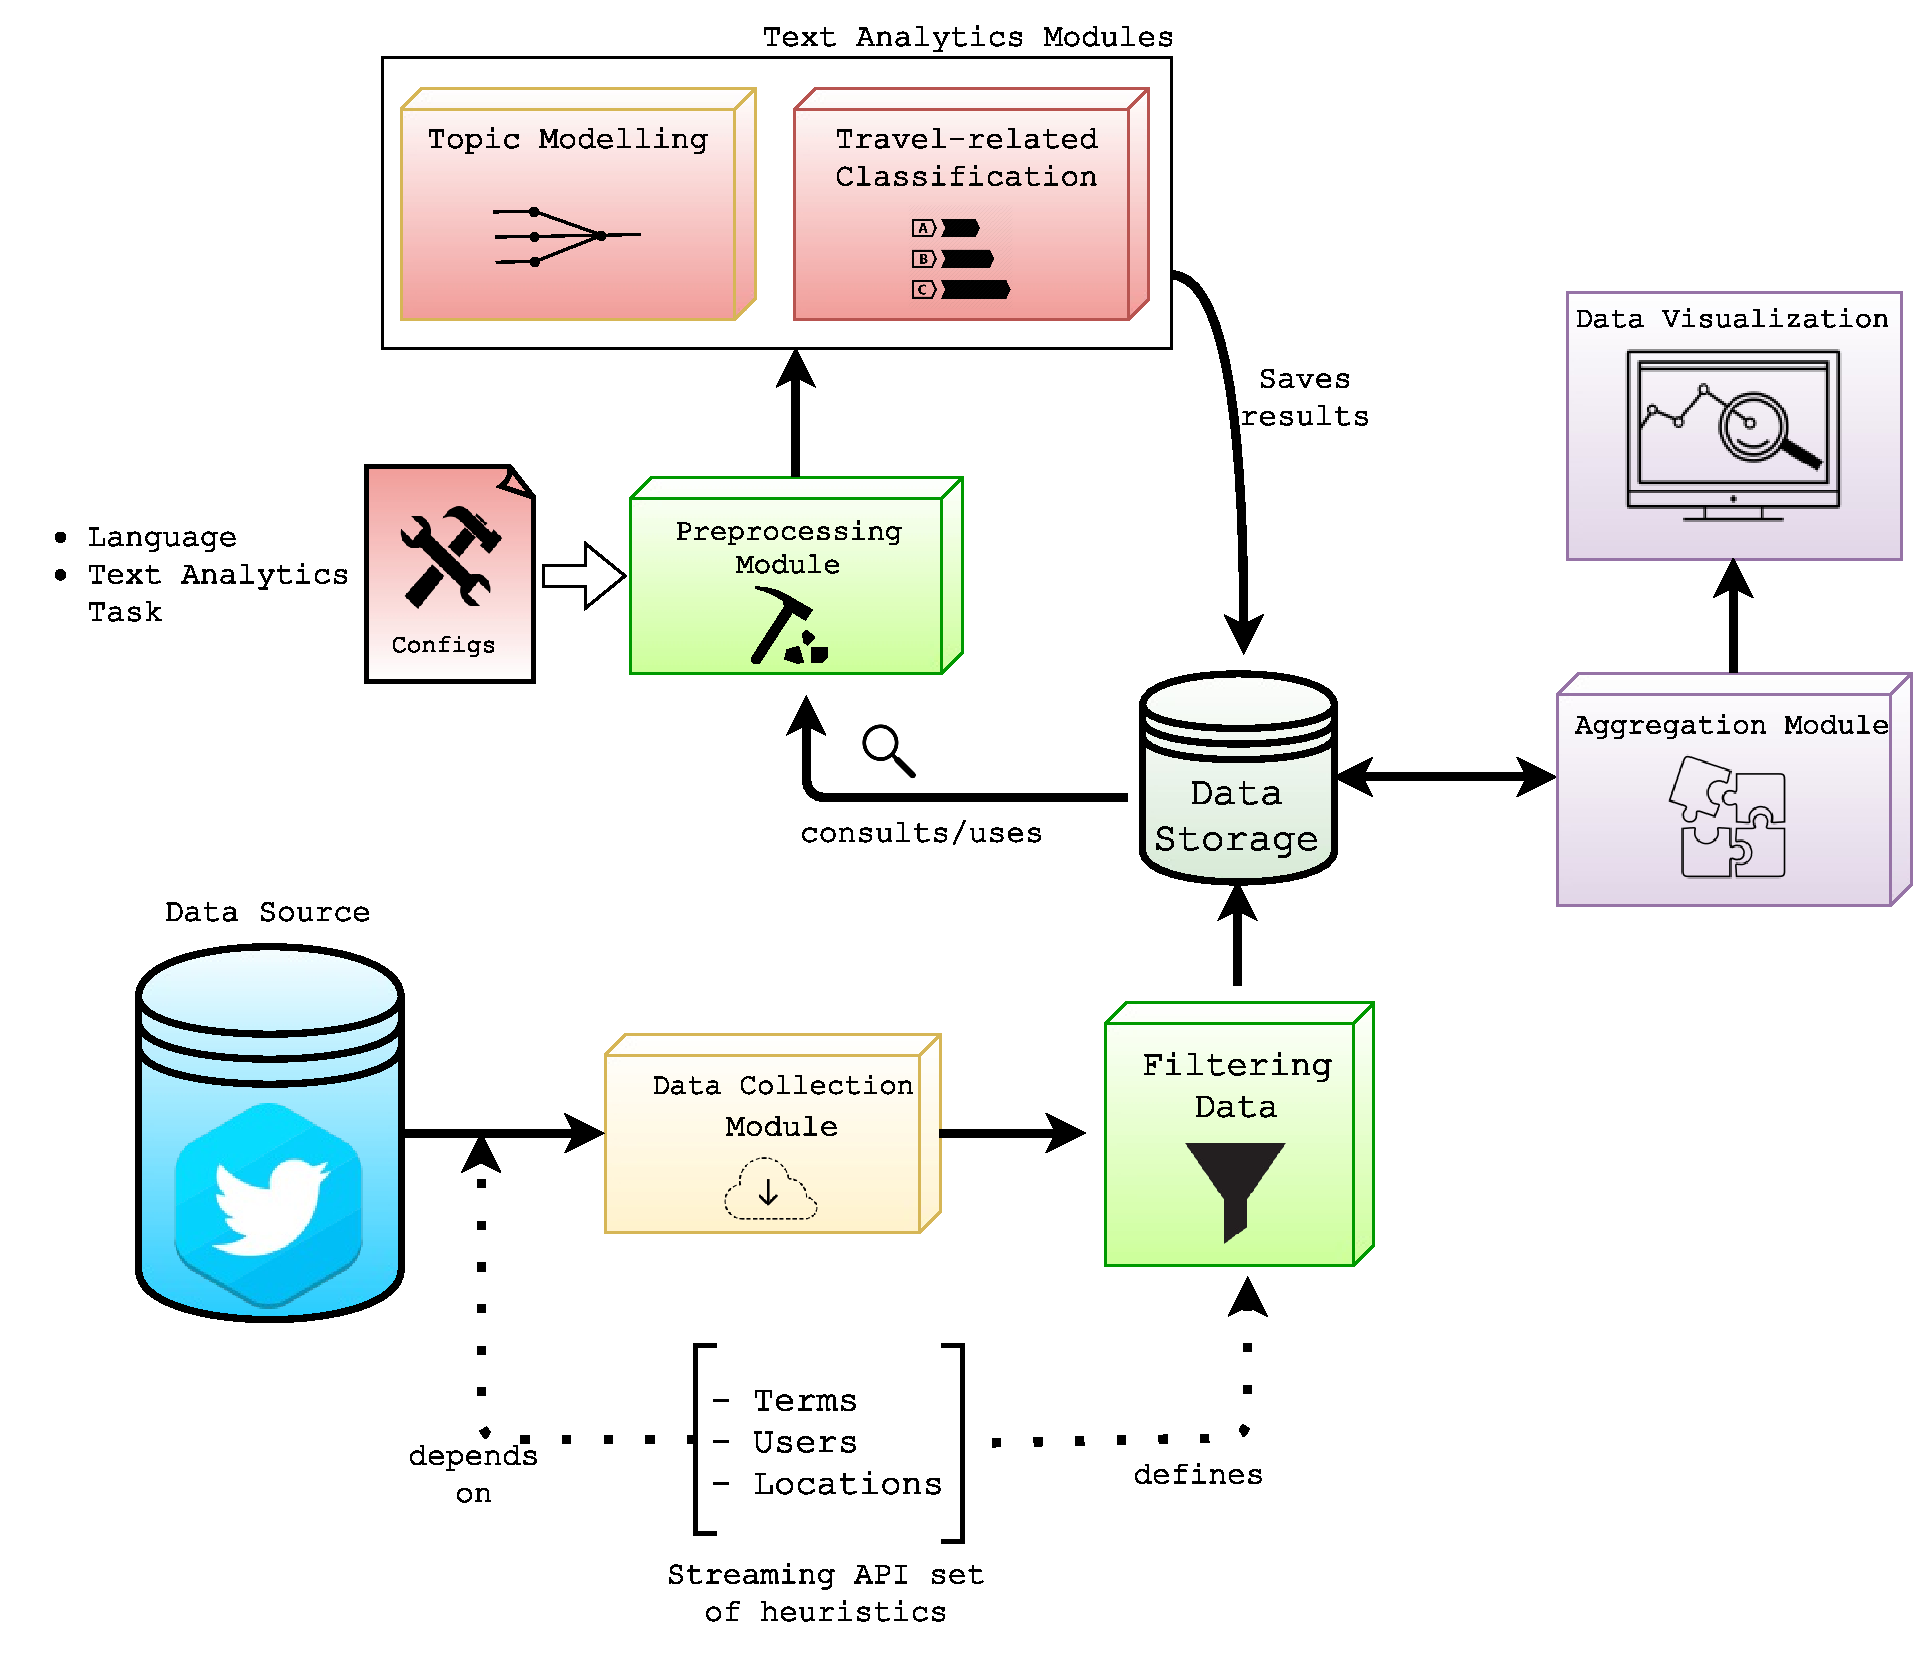
\includegraphics[width=\textwidth]{figures/architecture.pdf}
	\caption[Framework Architecture Overview]{Architecture overview of the proposed framework}
	\label{fig:architecture}
\end{figure}

\section{Data Collection}\label{sec:data_collection}

In Section~\ref{sec:requirements}, we explain the importance of the decision made to the data collection's heuristics. Twitter allows the developers' community two different tools to collect data, the Search and the Streaming APIs. The Search API is based on the RESTful protocol and only looks up for tweets published in the last 7 days, while the Streaming API creates basic endpoints (independent of the REST protocol) and retrieves up to 1\% of the Twitter Firehose~\footnote{Twitter Firehose - is a paid Twitter service that guarantees the delivery of 100\% of the tweets matched with certain criteria.}. Regarding the proposed and developed framework, we chose the Streaming API due to its free-access for the community, smooth integration in the module implementation and due to the availability of real-time information. A positive point about the Streaming API is the three available heuristics to the data collection, allowing the retrieval of tweets that match a specific text query (e.g. tweets with the word \texttt{bus} or \texttt{car}), the retrieval of tweets associated to a variable  number of users - being necessary previous knowledge about these users \textit{ids} - or even the retrieval of tweets located inside a bounding-box~\cite{mac2016effects}. There are two negative points regarding the Twitter Streaming API: first, Twitter imposes limits in its data exploration, where only 400 words can be tracked, 5,000 users can be followed and 25 different bounding-boxes can be explored\footnote{\url{https://dev.twitter.com/streaming/reference/post/statuses/filter} (Accessed on 18/06/2017)}; second, the previously mentioned heuristics cannot be used together, i.e. we can not track specific tweets from an user that match with certain words. Although the negative points, we remain with the choice made, of using the Twitter Streaming API as our source of information and limiting the heuristic to the one that retrieves tweets located inside a bounding-box. Our choice is additionally supported by the need of studying cities and exploring the information derived from it. This way, we know, a priori, that if the data collection method is able to retrieve tweets with precise geo-location then this makes our work easier since the exploration of specific regions of a city is already available taking into consideration the information available in tweets.

After the method selection, as well as the selection of its heuristic, we conduct an experiment regarding the amount of tweets being retrieved by one Twitter client for a city. Twitter has into consideration the number of clients used in the data collection process by tracking the IP address of the machine in the network. This constitutes a restriction to explore several cities with the same client since the Streaming API retrieves only 1\% of the total overcome. In the experiment, we tested the capacity of a client to retrieve all the tweets posted in New York City and used four different clients for it: one defined with the city bounding-box, and the other three defined with bounding-boxes of three boroughs in the city: Bronx, Brooklyn and Manhattan. Considering the bounding-boxes creation, we took support of an open-source \textit{online} tool coined BoundingBox~\footnote{\url{http://boundingbox.klokantech.com/} (Accessed on 23/06/2017)}, which is integrated with the Google Maps API.

Results showed that the client defined with the greatest bounding-box, New York City, was able to retrieve 100\% of the tweets from the three different boroughs. This experiment is consolidated with the work of F. Morstatter et al.~\cite{morstatter2013sample} where it was compared the Streaming API's capacity, regarding geo-located tweets, against the Twitter Firehose. Authors concluded that the percentage of geo-located tweets corresponds to 1-2\% of total overcome from Twitter and the Streaming API is able to retrieve almost 90\% of it. Hence, we do not need to be concerned about how many bounding-boxes are used in the collection process because if we did we would  need to be aware of 90\% of the world, which is not the case.

\section{Data Preprocessing}\label{sec:data_preprocessing}
The extraction of information from text, in particular from social media streams, is an iterative process and requires a segmented and planned pipeline to achieve the final results. In the requirements section (\ref{sec:requirements}), we mentioned some problems of social media streams as the short length and informality of the text message. The informality problem ranges from the writing style of each person to the existence of lots of abbreviations, slang, jargons, \textit{emoticons} and bad usage of punctuation signs. The preprocessing module presented in this section has as main goal the submission of the text messages under several operations in order to remove, or at least, reduce this type of informality characteristics and make easier the work of future tasks.

Below, we enumerate and described the different preprocessing methods implemented:

\begin{itemize}
	\item \textbf{Lower casing:} This operation is responsible for the conversion upper case characters to lower representation. The advantages provided by this operation are centered in the analysis of words written in different ways. An representative example is \texttt{london} and \texttt{London} whose meaning is the same but due to the different case in one letter, its representation/interpretation by text mining techniques may be disparate.
	\item \textbf{Tokenization:} Is the method of dividing each sentence in a list of tokens/words. Since we are dealing with social media content, standard tokenizations techniques available in packages, such as the \texttt{tokenize}~\footnote{\url{http://www.nltk.org/api/nltk.tokenize.html}} of NLTK Toolkit for Python, perform poorly and are not capable of dealing with \textit{\#hashtags}, \textit{@mentions}, abbreviations, strings of punctuation, \textit{emoticons} and unicode glyphs which are very common in Twitter. Having considered this, we used a Twitter-based tokenization package, coined Twokenize and firstly presented by B. O'Connor et al.~\cite{o2010tweetmotif}, which is capable of dealing with these special characteristics of tweets.
	\item \textbf{Punctuation Removal:} Depending on the future task, all signs of punctuation are removed. In this case, every \textit{emoticon} was removed, as well as the symbols \texttt{\#} and {@} which composed the \textit{hashtags} and user mentions.
	\item \textbf{User mentions and \textit{URLs} Removal:} Following the condition of the above mentioned operation, the removal from the text of this type of content depends of the current task.
	\item \textbf{Stop words Removal:} This operation consists in the removing of the most common words in the language in analysis. We used the standard words of the NLTK Corpus package.
\end{itemize}

Regarding other fields in a tweet, this module was also in charge of convert the date of creation of a tweet to the city timezone. The field \textit{created\_at} in a tweet is given in the Coordinated Universal Timezone (UTC) and in order to have knowledge about the most active local hours and days on Twitter, we used the Python timezone package \texttt{pytz} to convert the world timezone to the one desired.

Although the existence of more text preprocessing techniques, in this dissertation we only used the ones previously described since each of them is associated to, at least, one text analytics module whose are described in the following section.

\section{Text Analytics}
The extraction of information from texts can vary in several types depending on the task performed to achieve it. In this dissertation, it was developed different types of analysis having in consideration the text messages.

\subsection{Travel-related Classification}\label{sec:travel_classification}

\emph{Prima facie}, we tried to extract and characterize travel-related tweets from large datasets in order to study the geographical and temporal distributions of such specific content. To be successful in this task we create an automatic text classifier capable of discriminating travel-related tweets from non-related ones. Due to the absence of gold standard datasets in this domain, there was the need of creating a training and testing set of data in order to proceed the experiment and evaluate the performance of the obtained model. Conventional classification tasks in the domain of intelligent transportation systems follow traditional approaches by constructing their group of features using standard bag-of-words techniques. In our experiment, we tried to combine a bag-of-words technique with word embeddings methodologies, producing, for the best of our knowledge, the first travel-related classification model with both type of features.

The word embeddings technique is used by T. Mikolov~et~al.~\cite{mikolov2013efficient} in the implementation of a powerful computational method named \emph{word2vec}. This method is capable of learning distributed representations of words, and each word is represented by a distribution of weights across a fixed number of dimensions. Authors have also proved that such representation is robust when encoding syntactic and semantic similarities in the embedding space.

The training objective of the skip-gram model, as defined by T. Mikolov~et~al.~\cite{mikolov2013linguistic}, is to learn the target word representation, maximizing the prediction of its surrounding words given a predefined context window. For instance, to the word $w_t$, present in a vocabulary, the objective is to maximize the average log probability:

\begin{equation}
\frac{1}{T}  \sum_{t=1}^{T}  \sum_{-c \leq j \leq  c, j \neq 0} \textnormal{log } P(w_{t+j} | w_t)
\end{equation}

where $c$ is the size of the context window, $T$ is the total number of words in the vocabulary and $w_{t+j}$ is a word in the context window of $w_t$. After training, a low dimensionality embedding matrix $\textbf{E}$ encapsulates information about each word in the vocabulary and its use (i.e. the surrounding contexts). For instance, by using the skip-gram model over our datasets we were able to verify that words such as \texttt{ônibus} and \texttt{busão} are used in the similar contexts, as a mode of transport.

Later on, Q. Le and T. Mikolov~\cite{le2014distributed} developed paragraph2vec, an unsupervised learning algorithm operating on pieces of text not necessarily of the same length. The model is similar to \emph{word2vec} but learns distributed representations of sentences, paragraphs or even whole documents instead of words. We used \emph{paragraph2vec} to learn the vector representations of each tweet and tried several configurations in the model hyper-parameterization.

The previous described methods are available in the collection of Python scripts we used in this dissertation, coined \texttt{Gensim}~\footnote{\url{https://radimrehurek.com/gensim/about.html} (Accessed on 20/06/2017)}, presented and lately improved by R. \v{R}eh\r{u}\v{r}ek and P. Sojka~\cite{rehurek2010software}.

The overall experiment regarding the travel-related classification of tweets is described and detailed in Section~\ref{sec:travel_related_classification}. Concluded the experiment, we select the best classifier and used it the implementation of the travel-related module allowing the framework to discriminate potential new tweets related to the transportation domain.

\subsection{Topic Modelling}\label{sec:topic_modelling}

Further developments towards the enrichment of different information provided by the framework took us to the path of topic modelling techniques for text messages. Topic modelling is a text mining technique which goal is the identification of latent topics in a collection of documents. During the last decade, the research community had been using this technique in a vast range of works aiming the test of its applicability in different domains. Here, we also used topic modelling to characterize the different cities and provide this type of information to the framework's end-users.

Latent Dirichlet Allocation (LDA) is a generative statistical model proposed by D. Blei et al.~\cite{blei2003latent} that makes possible the discovering of unknown groups and its similarities over a collection of text documents. The model tries to identify what topics are present in a document by observing all the words that composing it, producing as final result a topic distribution. 

\begin{figure}[htbp]
	\centering
	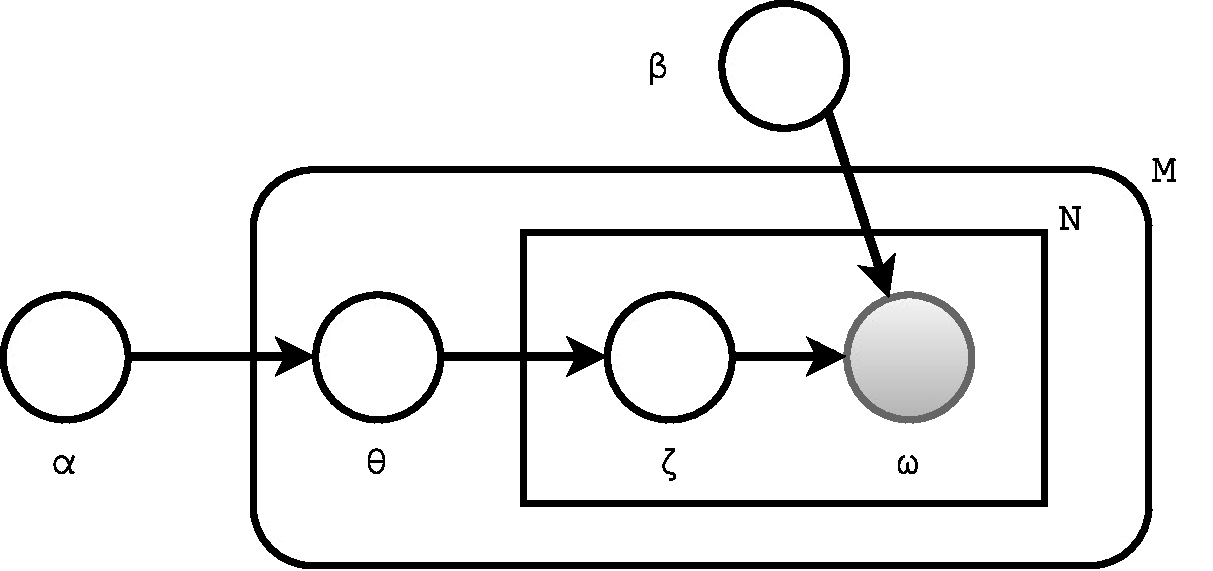
\includegraphics[scale=0.41, keepaspectratio]{figures/lda-model.pdf}
	\caption[Plate notation of LDA by D.Blei et al. ~\cite{blei2003latent}]{Plate Notation of the graphical model representation of Latent Dirichlet Allocation by D.Blei et al. ~\cite{blei2003latent}}
	\label{fig:lda_graphical_model_representation}
\end{figure}

In Figure~\ref{fig:lda_graphical_model_representation} it is illustrated the plate notation to the graphical model of LDA. There, we can observe that for a collection of documents $M$, each one composed by a sequence of $N$ words, the model tries to attribute a per-document topic distribution, using an $\alpha$ dirichlet prior, to a topic-word distribution $\xi$ (associated also with a dirichlet prior $\beta$), inducing that each topic's probability $\theta$ is focused in a small set of words $w$ which characterize that topic.

The most important advantage this model provides is related to the group of features involved in its training process. Conventional application of this model uses only as features a bag-of-words matrix representation~\footnote{Bag-of-words representation matrix is a list of lists, where each entry of the matrix is associated to a sentence of the document and takes the form of a term-frequency vector.}, and for this reason the task of topic modelling becomes very simple since the the frequency of words in the documents are taken into account. Last but not least, LDA model performs two different distributions: (1) distribution of words over topics and (2) distribution of topics over the documents, resulting in the assumption that each document is random mixture of topics, whose in turn are composed by a probabilistic distribution of words.

The cities' characterization provided by our framework centers in the topics being talked about at the time. We conduct an experiment to evaluate if such information could bring added-value for the cities entities and the results although being very promiscuous proved to have potential in certain occasions. The overall experiment is described in Section~\ref{sec:topic_modeling} as well as potential improvements to the generated model.

\subsection{Final Remarks}

The previous mentioned text analytics methodologies were implemented as separate modules in the framework since each of them needs different preprocessing operations over the data. A future interesting improvement to the framework, presented in this dissertation, is the incorporation of an extra module of sentiment analysis that should work together with the two already developed, and provide additional information about the services of a smart city, including the transportation domain.

\section{Data Storage and Aggregation}\label{sec:storage_aggregations}

Besides the few percentage of geo-located tweets provided by Twitter (1-2\% of the total Firehose overcome), this data requires, in the first place, large physical space for storage and, secondly, a tool that allows the easy manipulation and quick access of data. Having considered this, we opted for the use MongoDB, an open-source cross-platform document-oriented database, as the database system for our framework. MongoDB allows the storage of JSON-like documents which is the retrieved format of tweets by the Streaming API. Since in this dissertation we developed the framework as a prototype of a system capable of extracting information related to \textit{smart cities} and transportation services, the large physical space to storage data was not a priority.

MongoDB presents, alongside the high performance, availability and scaling, an inner framework that allows the aggregation of data according to specific user-generated queries. Here, we took advantage of such a pipeline in order to produce interesting statistics regarding the processed data. Map-reduce is the processing paradigm behind the aggregating operations allowing high performance even when applied to large volumes of data, as in this particular case where it is necessary to process thousands or millions of tweets in a short period of time.

\section{Visualization}\label{sec:visualization}

One of the most laborious and time-consuming tasks in the development of this social media based framework was the selection of data visualizations to illustrate the results provided by the previous mentioned modules. Due to the amount of data being processed, the generation of data visualization using an atomic implementation is sometimes poorly in terms of response time. Hence, we needed to adopt a different approach in order to solve this non-efficient procedure.

After a long period of research, we found a solution to this problem by creating a set of routines (bash scripts) that are called periodically (hourly) to execute all type of necessary aggregations and update its corresponding data collections in the database. Then, other routine is invoked to generate all type of data visualizations and store its visual representation in HTML files. In the implementation of this module, these files - containing the data visualization - were embedded inside several view pages. \texttt{Plotly}~\footnote{\url{https://plot.ly/python/}} is a Python graphing library that has available the saving of the visualizations produced in files with HTML format. Besides that, the library offers an extensive range of graphical representations, such as basic charts (bar charts, scatter plots, etc), scientific charts (heatmaps), financial charts (time series) and maps (choropleth, bubble and line maps), which facilitates the construction and designing of dynamic dashboards. Here, we explore mostly the section of basic charts to build simple representations of the results obtained from the analytics phase and also added top lists about some metadata of the tweets, as so the overall, daily and hourly top \textit{hashtags} and uni-grams.

%\section{Summary}
\chapter{Implementação}\label{chap:chap4}

\section*{}

Este capítulo pode ser dedicado à apresentação de detalhes de nível
mais baixo relacionados com o enquadramento e implementação das
soluções preconizadas no capítulo anterior.
Note-se no entanto que detalhes desnecessários à compreensão do
trabalho devem ser remetidos para anexos.

Dependendo do volume, a avaliação do trabalho pode ser incluída neste
capítulo ou pode constituir um capítulo separado.

\section{Secção Exemplo}

%\todofigure{Inserir uma figura sobre o Map/Reduce}

Lorem ipsum dolor sit amet, consectetuer adipiscing elit. Integer
hendrerit commodo ante. Pellentesque nibh libero, aliquam at, faucibus
id, commodo a, velit. 
%\todoline{Escrever sobre o map/reduce}
Duis eleifend sem eget leo. Morbi in est. Suspendisse magna sem,
varius nec, hendrerit non, tincidunt quis, quam. Aenean congue. 
%\todolines{A short entry in the list of todos}{A very long todonote
%  that certainly will fill more than a single line in the list of
%  todos. Just to make sure let's add some more text.} 
Vivamus vel est sit amet sem iaculis posuere. Cras mollis, enim vel
gravida aliquam, libero nunc ullamcorper dui, ullamcorper sodales
lectus nulla sed urna. Morbi aliquet porta risus. 
Proin vestibulum ligula a purus. Maecenas a nulla. 
Maecenas mattis est vitae neque auctor tempus. Etiam nulla dui,
mattis vitae, porttitor sed, aliquet ut, enim. Cras nisl magna,
aliquet et, laoreet at, gravida ac, neque. Sed id est. Nulla dapibus
dolor quis ipsum rhoncus cursus. 

\section{Mais uma Secção}

Lorem ipsum dolor sit amet, consectetuer adipiscing elit. Quisque
purus sapien, interdum ut, vestibulum a, accumsan ullamcorper,
erat. Mauris a magna ut leo porta imperdiet. Donec dui odio, porta in,
pretium non, semper quis, orci. Quisque erat diam, pharetra vel,
laoreet ac, hendrerit vel, enim. Donec tristique luctus risus. Fusce
dolor est, eleifend id, elementum sit amet, varius vitae, neque. Morbi
at augue. Ut sem ligula, auctor vitae, facilisis id, pharetra non,
lectus. Nulla lacus augue, aliquam eget, sollicitudin sed, hendrerit
eu, leo. Suspendisse ac tortor. Mauris at odio. Etiam vehicula. Nam
lacinia purus at nibh. Aliquam fringilla lorem ac justo. Ut nec
enim. 
%\todoref{Citar Map/reduce}

Quisque ullamcorper. Aliquam vel magna. Sed pulvinar dictum
ligula. Sed ultrices dolor ut turpis. Vivamus sagittis orci malesuada
arcu venenatis auctor. Proin vehicula pharetra urna. Aliquam egestas
nunc quis nisl. Donec ullamcorper. Nulla purus. Ut suscipit lacus
vitae dui. Mauris semper. Ut eget sem. Integer orci. Nam vitae dui
eget nisi placerat convallis. 

\begin{lstlisting}[float,language=Java, label=src:mapreduce, caption=Example map and reduce functions for word counting]
map(String key, String value): 
// key: document name 
// value: document contents 
for each word w in value:
EmitIntermediate(w, "1");

reduce(String key, Iterator values):
// key: a word 
// values: a list of counts 
int result = 0;
for each v in values: 
result += ParseInt(v);

Emit(AsString(result))
\end{lstlisting}

Sed id lorem. Proin gravida bibendum lacus. Sed molestie, urna quis
euismod laoreet, diam dolor dictum diam, vitae consectetuer leo ipsum
id ante. Integer eu lectus non mauris pharetra viverra. In feugiat
libero ut massa. Morbi cursus, lorem sollicitudin blandit semper,
felis magna pellentesque lacus, ut rhoncus leo neque at tellus. Sed
mattis, diam eget eleifend tincidunt, ligula eros tincidunt diam,
vitae auctor turpis est vel nunc. In eu magna. Donec dolor metus,
egestas sit amet, ultrices in, faucibus sed, lectus. Etiam est enim,
vehicula pharetra, porta non, viverra vel, nunc. Ut non sem. Etiam nec
neque. 

\section{Resumo ou Conclusões}

Proin vehicula pharetra urna. Aliquam egestas
nunc quis nisl. Donec ullamcorper. Nulla purus. Ut suscipit lacus
vitae dui. Mauris semper. Ut eget sem. Integer orci. Nam vitae dui
eget nisi placerat convallis. 

\chapter{Conclusões e Trabalho Futuro} \label{chap:concl}

\section*{}

Deve ser apresentado um resumo do trabalho realizado e apreciada a
satisfação dos objetivos do trabalho, uma lista de contribuições
principais do trabalho e as direções para trabalho futuro.

A escrita deste capítulo deve ser orientada para a total compreensão
do trabalho, tendo em atenção que, depois de ler o Resumo e a
Introdução, a maioria dos leitores passará à leitura deste capítulo de
conclusões e recomendações para trabalho futuro.

\section{Conclusão}

\subsection{Possíveis Vantagens e Desvantagens}

\section{Trabalho Futuro}

\subsection{Planeamento do Desenvolvimento}

\vspace*{12mm} 


%%----------------------------------------
%% Final materials
%%----------------------------------------

%% Glossary / Nomenclature
\nomenclature{IQR}{\textbf{I}nter\textbf{q}uatile \textbf{R}ange}, being equal to the difference between 75th and 25th percentiles, or between upper and lower quartiles, $IQR = Q3 −  Q1$
\printnomenclature[4.5cm]

%% Bibliography
%% Comment the next command if BibTeX file not used
%% bibliography is in ``myrefs.bib''
\PrintBib{myrefs}

%% comment next 2 commands if numbered appendices are not used
\appendix
\chapter{Loren Ipsum} \label{ap1:loren}

Depois das conclusões e antes das referências bibliográficas,
apresenta-se neste anexo numerado o texto usado para preencher a
dissertação.

\section{O que é o \emph{Loren Ipsum}?}

\emph{\textbf{Lorem Ipsum}} is simply dummy text of the printing and
typesetting industry. Lorem Ipsum has been the industry's standard
dummy text ever since the 1500s, when an unknown printer took a galley
of type and scrambled it to make a type specimen book. It has survived
not only five centuries, but also the leap into electronic
typesetting, remaining essentially unchanged. It was popularised in
the 1960s with the release of Letraset sheets containing Lorem Ipsum
passages, and more recently with desktop publishing software like
Aldus PageMaker including versions of Lorem Ipsum~\citep{kn:Lip08}. 

\section{De onde Vem o Loren?}

Contrary to popular belief, Lorem Ipsum is not simply random text. It
has roots in a piece of classical Latin literature from 45 BC, making
it over 2000 years old. Richard McClintock, a Latin professor at
Hampden-Sydney College in Virginia, looked up one of the more obscure
Latin words, consectetur, from a Lorem Ipsum passage, and going
through the cites of the word in classical literature, discovered the
undoubtable source. Lorem Ipsum comes from sections 1.10.32 and
1.10.33 of ``de Finibus Bonorum et Malorum'' (The Extremes of Good and
Evil) by Cicero, written in 45 BC. This book is a treatise on the
theory of ethics, very popular during the Renaissance. The first line
of Lorem Ipsum, ``Lorem ipsum dolor sit amet\ldots'', comes from a line in
section 1.10.32.

The standard chunk of Lorem Ipsum used since the 1500s is reproduced
below for those interested. Sections 1.10.32 and 1.10.33 from ``de
Finibus Bonorum et Malorum'' by Cicero are also reproduced in their
exact original form, accompanied by English versions from the 1914
translation by H. Rackham.

\section{Porque se usa o Loren?}

It is a long established fact that a reader will be distracted by the
readable content of a page when looking at its layout. The point of
using Lorem Ipsum is that it has a more-or-less normal distribution of
letters, as opposed to using ``Content here, content here'', making it
look like readable English. Many desktop publishing packages and web
page editors now use Lorem Ipsum as their default model text, and a
search for ``lorem ipsum'' will uncover many web sites still in their
infancy. Various versions have evolved over the years, sometimes by
accident, sometimes on purpose (injected humour and the like). 

\section{Onde se Podem Encontrar Exemplos?}

There are many variations of passages of Lorem Ipsum available, but
the majority have suffered alteration in some form, by injected
humour, or randomised words which don't look even slightly
believable. If you are going to use a passage of Lorem Ipsum, you need
to be sure there isn't anything embarrassing hidden in the middle of
text. All the Lorem Ipsum generators on the Internet tend to repeat
predefined chunks as necessary, making this the first true generator
on the Internet. It uses a dictionary of over 200 Latin words,
combined with a handful of model sentence structures, to generate
Lorem Ipsum which looks reasonable. The generated Lorem Ipsum is
therefore always free from repetition, injected humour, or
non-characteristic words etc. 


%% Index
%% Uncomment next command if index is required
%% don't forget to run ``makeindex mieic-en'' command
%\PrintIndex

\end{document}
